\section{Analysis}

\subsection{Photodetector position} \label{mppcposition}
The location of each photodetector is determined using charge
generated in the photodectectors by X-ray interactions corresponding
to a precisely placed source.  An outline of the detector is created
by X-ray events and fitted to determine the center position (fig
\ref{fig:xraycharge}). 

\begin{figure}[h]
  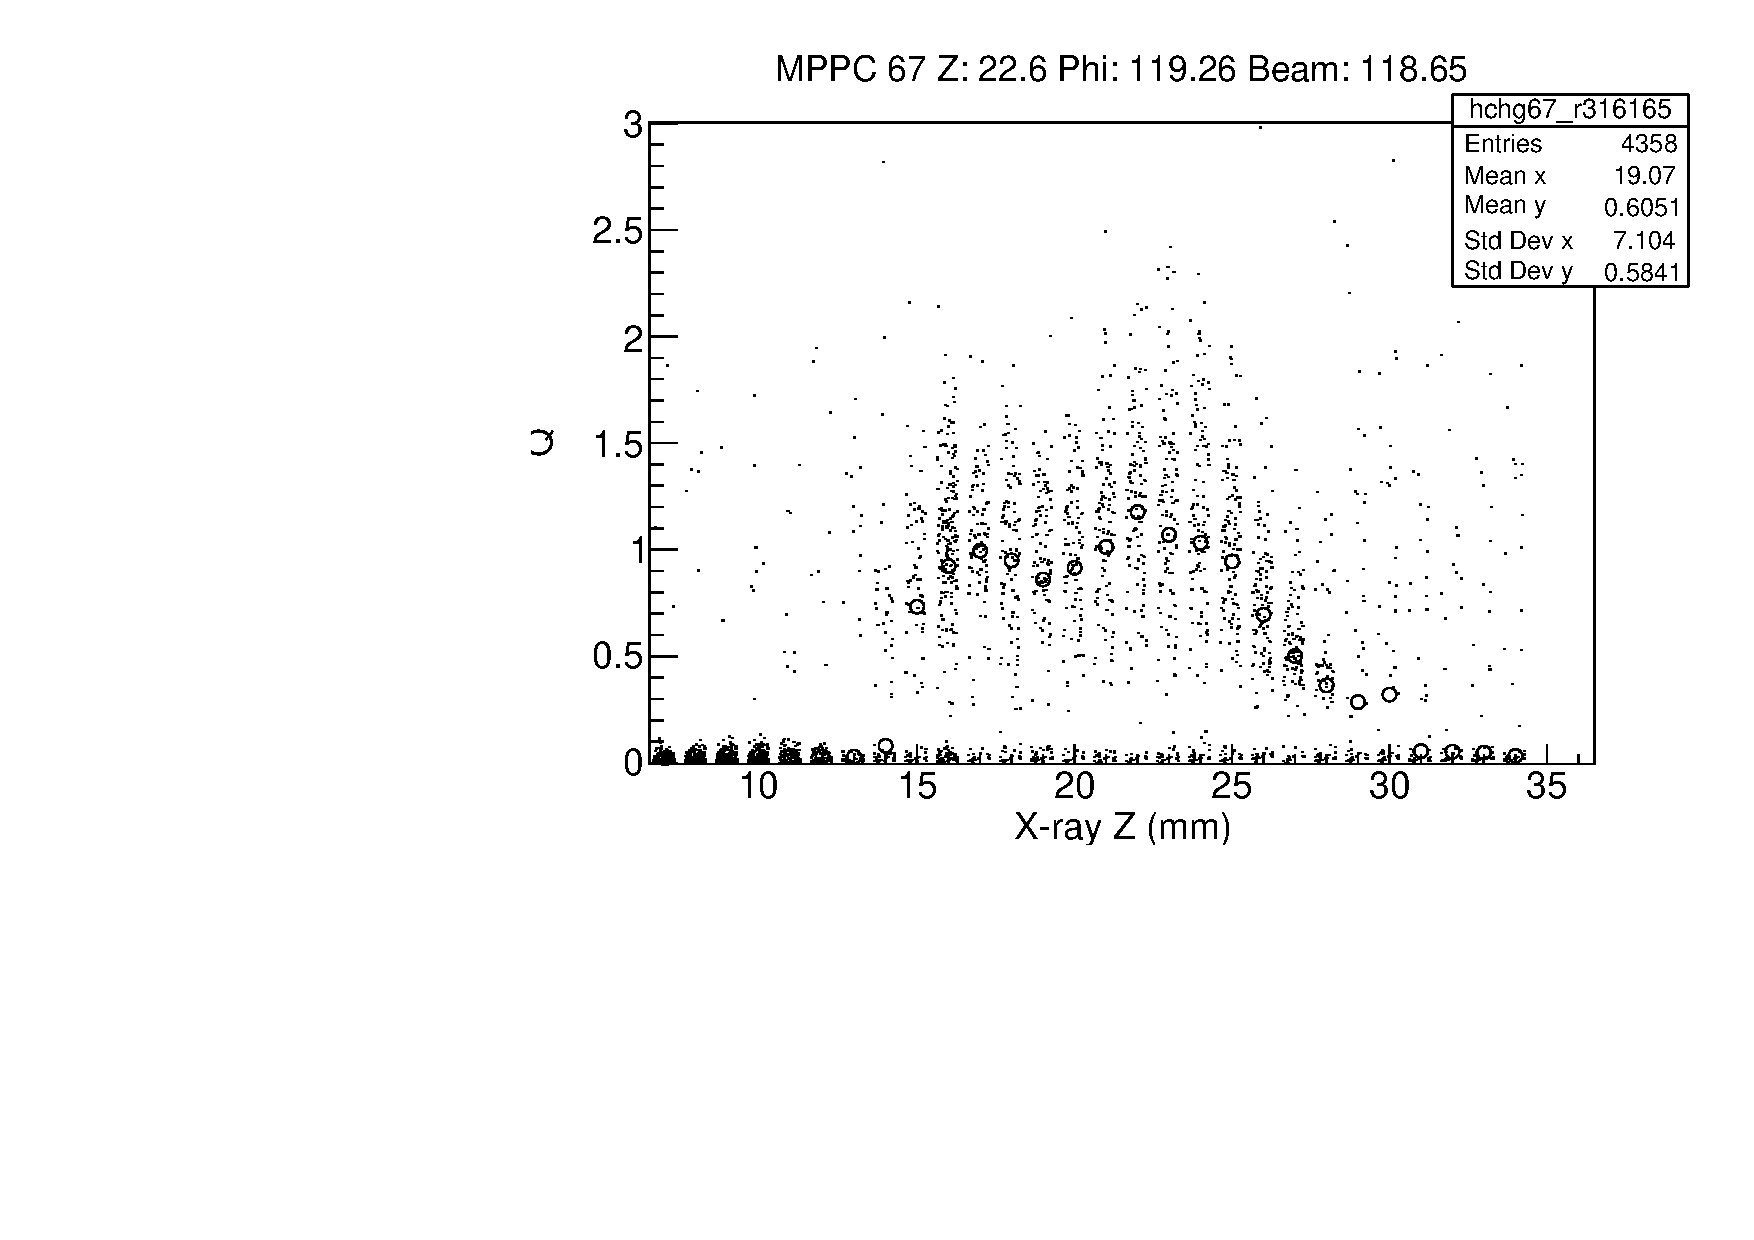
\includegraphics[width=4cm]{plots/2018/hcharge67_z}
  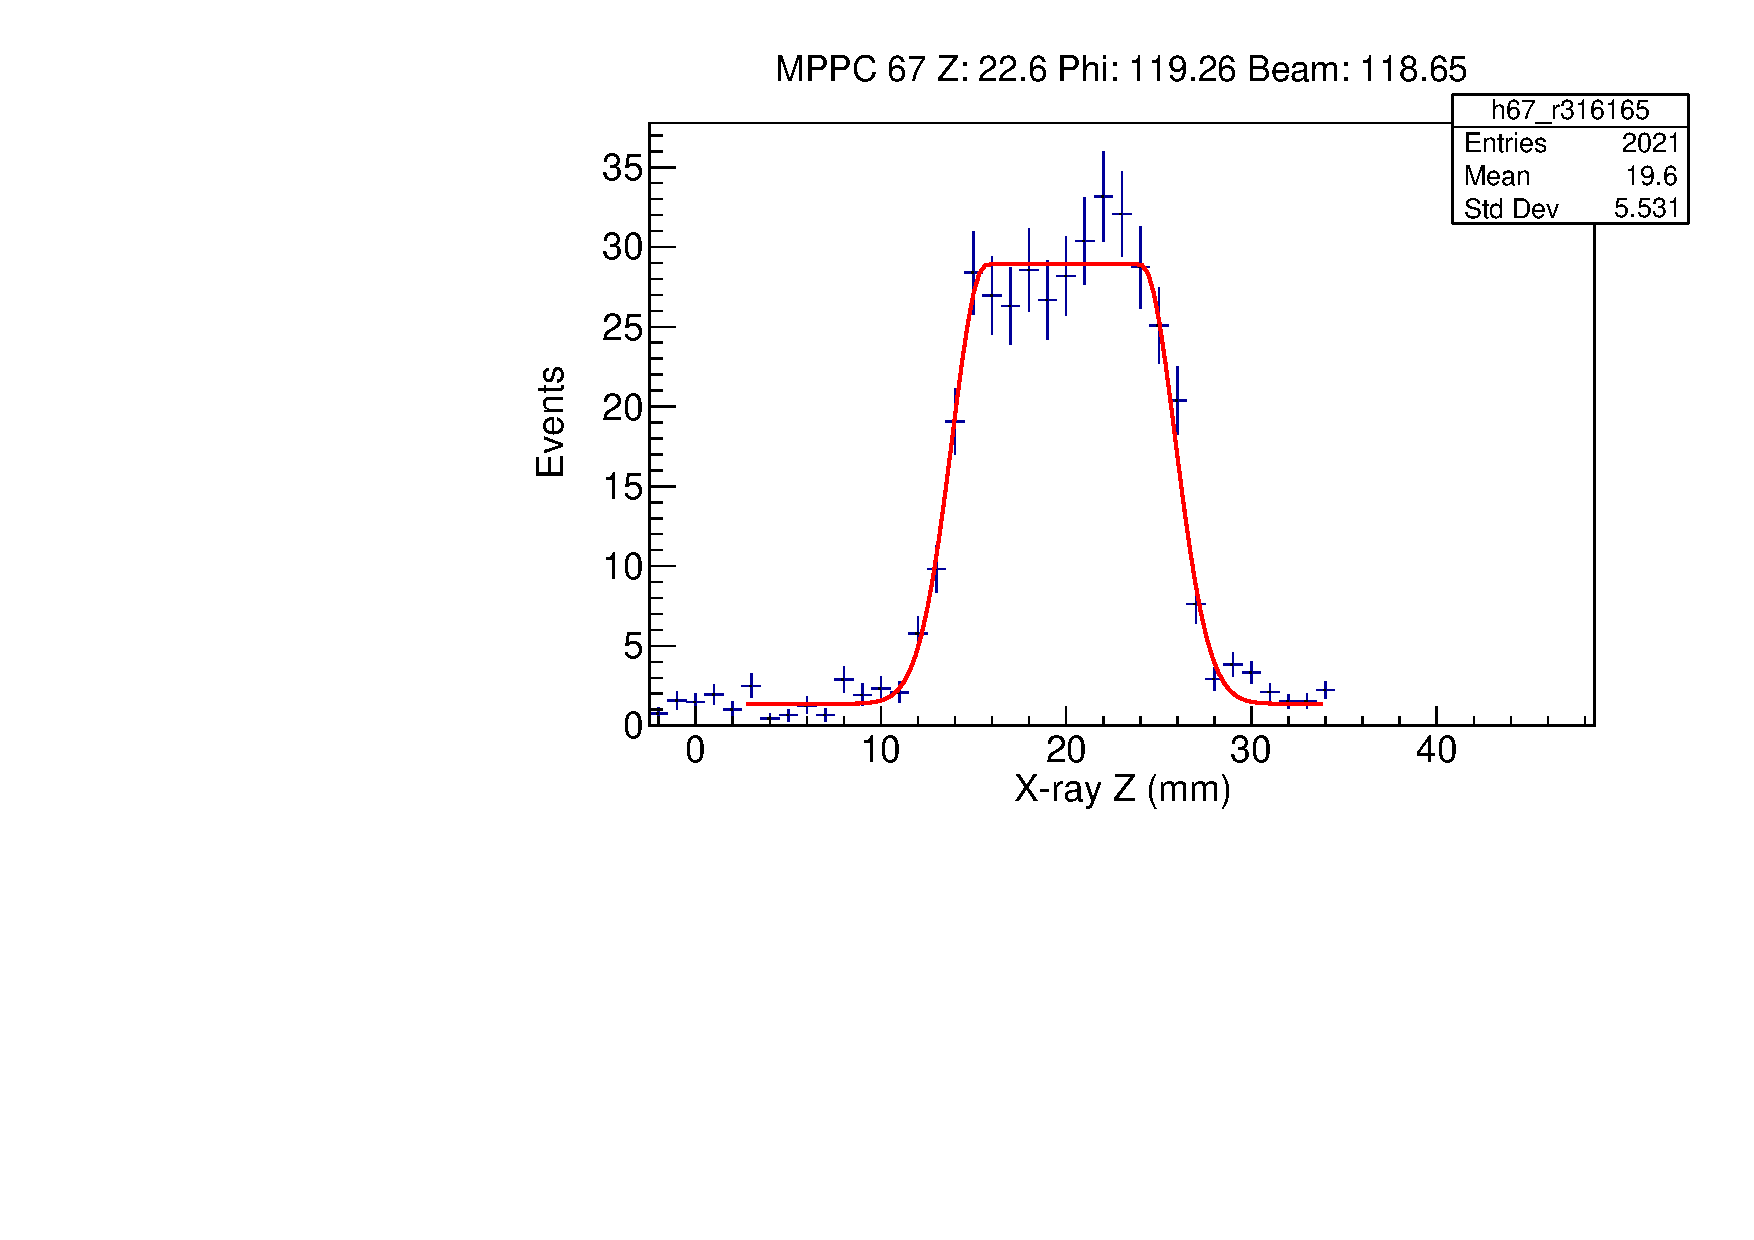
\includegraphics[width=4cm]{plots/2018/mppc_fit}
  \caption{Charge recorded in a single photodetector as a function of X-ray Z coordinate 
  (left) and 
    the calculated event rate (right).}
  \label{fig:xraycharge}
\end{figure}  

To isolate signal events, a trigger threshold on cumulative charge 
in the region of scanned photodetectors is applied with background 
subtraction to exclude coherent electronic noise. Additionally, 
an offline selection criteria matching X-ray energy pattern are applied
requiring large relative and absolute charge in the channel with highest charge
($>70\%$,$>0.4$~pC) and simultaneously a small deposition 
in the rest of the channels ($<0.1$~pC, and second highest charge$<10\%$).

The X-ray event rate as a function of X-ray position ($z$/$\phi$) is
fitted with the following piece-wise continuous function,
\begin{equation} \label{eqn:linetwogaus}
    f(z) = 
    \begin{cases}
        b+s\cdot e^{-\frac{(z - \, (\mu_m - w/2)\, )^2}{\sigma_m^2}} & z < \mu_m-w/2     \\
        b+s\cdot e^{-\frac{(z - \, (\mu_m + w/2)\, )^2}{\sigma_m^2}} & z > \mu_m+w/2     \\
        b+s                                         & \mu_m - w/2 < z < \\
                                               & \mu_m + w/2    \\
    \end{cases}
\end{equation}
where $w$ and $\mu_{m}$ are the width and center position of
the photodetector, $\sigma_{m}$ gaussian width of the edges, and $s,\,b$
are the signal and background event rates. Additionally, a supplemental 
analysis was conducted using a supergaussian function for fitting the
event rate.\\
\begin{equation} \label{eqn:supergaus}
    f(z)=b+s\cdot Exp\left[-\left(\frac{z-\mu_{m}}{\sigma_{w}}\right)^{8}\right]
\end{equation}
A sample of well fit photodetector locations -- from both fitting functions -- is used for  subsequent analysis.


%\subsection{Photodetector Properties}
%The entrance face of the LXe calorimeter consists of 4092 MPPCs
%arranged in a grid structure containing 93 rows in the $\phi$ direction.  
%A row consists of 44 MPPCs placed along $Z$ direction, divided equally in two
%PCB\footnote{Printed Circuit Board} strips on the upstream and
%downstream side of the calorimeter \cite{megdesign}.  The PCB strips
%are mounted with spacer materials on four CFRP\footnote{Carbon Fiber
%Reinforced Polymer} plates, each containing 23-24 strips and attached
%to the inner face of the cryostat at different $\phi$ locations.  The
%in-situ position and alignment of the MPPCs and its installation
%assembly is verified in the following sections.


\subsection{Photodetector Properties} \label{mppcproperties}
The entrance face of the LXe calorimeter consists of 4092 MPPCs
arranged in a grid structure containing 93 rows in the $\phi$ direction.  
A row consists of 44 MPPCs placed along $Z$ direction, divided equally in two
PCB\footnote{Printed Circuit Board} strips on the upstream and
downstream side of the calorimeter \cite{megdesign}.  The PCB strips
are mounted with spacer materials on four CFRP\footnote{Carbon Fiber
Reinforced Polymer} plates, each containing 23-24 strips and attached
to the inner face of the cryostat at different $\phi$ locations.  The
in-situ position and alignment of the MPPCs and its installation
assembly is verified in the following sections.



\noindent {\bf Spacing in Z and $\phi$}\\
The photodetectors are manufactured and assembled in lattice formation
to high precision, which can be used for validation of the X-ray
scanning technique and calculate its resolution.  A change in the
spacing can also reveal the effect of thermal cooling as well as
installation errors.  The spacing between individual MPPC pairs as
well as mean spacing between adjacent MPPC is calculated per PCB strip
(row-wise) along Z and per cfrp plate (column-wise) along \phis. 

Table \ref{tab:oddeven} shows spacing between individual MPPC pairs separated
into two groups which include alternate pairs along columns for Z measurement,
and rows for \phis measurement.  Nominally we expect the spacing to be equal in
the two groups; the data shows the spacing in Z coordinate differs by 0.88~mm
and 0.74~mrad in the $\phi$ coordinate.  
The average spacing (shown in table \ref{tab:avgspacing}), however is 
consistent with expectation after accounting
for thermal cooling suggests no cumulative effect. 
This implies that individual MPPC position is systematically
shifted or miscalculated by 0.22~mm (0.18 mrad), and varying 
perdiocally with the phase of $\sim$ 30~mm, or two MPPC widths. 
The source of this discrepancy is not known.
The possible cause due to inaccurate corrections to X-ray position
is considered but ruled out as periodicity of the corrections does not
match that of the observed effect; Z corrections have a period 
of 100~mm while $\phi$ corrections are monotonic.

Although the systematic shift seen in pairwise MPPC spacing is small compared
to the overall measurement uncertainty, its effect on the photon position
resolution is estimated using MC simulation.  
A signal photon
interaction (E$_\gamma$=53~MeV) 
is simulated at a normal distance equivalent to 
one radiation length ($\lambda_{LXe}\approx$ 2.75 cm) 
over a two dimensional surface 
consisting of (20$\times$20) photodetector array. 
The isotropic distribution of photons generated as a result
is recorded by the photodetector array. The signal in each 
photodetector is proportional to the solid angle subtended to the
interaction point, and detection efficiency determined by the
photon incident angle.
The dimensions and spacing of the photodetectors are identical to
the MPPC in the calorimeter. Each event is simulated with
an interaction point chosen randomly in a 30$\times$30~mm$^2$
region equivalent to two MPPC widths, 
and reconstructed twice with nominal and systematically
shifted photodetector positions by 0.22~mm. 
The photon position is reconstructed using weighted mean 
of the signal recorded in the photodetectors.

[Results of test simulation]\\


The mean distance between adjacent MPPCs is calculated
using only the measurements at the 
end of the row or column.
The precision of the measurement is improved as a result compared to the
pair-wise spacing by  one (two) order of magnitude in Z ($\phi$).  In
the Z coordinate, the mean distance is calculated for each PCB strip
as well as for the half-strips (US and DS) connected at the center.
Similarly in the $\phi$ coordinate, the mean distance is calculated
within individual cfrp plates and overall.  The mean and standard
deviation of the calculated mean distance in Z and $\phi$  show a
regular grid structure with no deformation in the scanned region
(table \ref{tab:avgspacing}).

The effect of thermal cooling is seen in Z with the
mean distance 15.08~mm  or 30~\micron contraction between adjacent
MPPCs. The mean distance in $\phi$ is dependent on the X-coordinate of
the semi-cylindrical LXe calorimeter whose center is nominally aligned
with the center of the X-ray scanning device.  During the X-ray survey
the calorimeter was off-center, shifted towards the X-ray device by
3.85~mm increasing the mean angular spacing seen in the data.  The
following sections detail the qualitative use of X-ray data to measure
thermal contraction and 3d MPPC location.

\begin{table}
\begin{tabular}{ccccc}
 & $Z_{n} - Z_{n-1}$ &Std. Dev.& $\phi_{n} - \phi_{n-1}$ & Std. Dev. \\
 & [mm] &[mm]& [mrad]& [mrad]\\
\hline
Odd  $n$ & 15.69 & 0.49 & 24.12 & 0.54 \\ 
Even $n$ & 14.57 & 0.57 & 23.38 & 0.70 \\ 
%Nominal  & 15.1  &      & 23.55 & \\
\end{tabular}
\caption{Mean Z and $\phi$ spacing calculated for Odd-Even and Even-Odd
combination  of adjacent MPPCs.}
\label{tab:oddeven}
\end{table}

\begin{table}
\begin{tabular}{clc}
   & Z [mm] &Std. Dev. [mm] \\
\hline
US     & 15.091(32)& 0.127  \\
DS     & 15.101(49)& 0.164  \\
All    & 15.081(8) & 0.061  \\
Nominal& 15.1      &
\end{tabular}

\begin{tabular}{clc}
   & $\phi$ [mrad] &Std. Dev. [mrad] \\
\hline
cfrp 1     & 23.733(13)& 0.032  \\
cfrp 2     & 23.716(15)& 0.055  \\
cfrp 3     & 23.689(12)& 0.035  \\
cfrp 4     & 23.727(11)& 0.037  \\
All        & 23.725(2) & 0.008  \\
Nominal    & 23.55 &     
\end{tabular}
\label{tab:avgspacing}
\caption{Mean distance between adjacent MPPC calculated over the entire row (Z) or 
column ($\phi$). Upstream (US) and downstream (DS) parts of each PCB strip, and
individual cfrp plates are calculated separately, and altogether.}
\end{table}


\noindent {\bf R coordinate calculation}\\
The radial coordinate not directly measured in the X-ray scan can be
calculated using information from the FARO scan of the photodetectors.
The FARO scan provides highly precise ($\sigma_{|\vec{x}|}$ = 200
\micron) 3D coordinates of a subset of photodetectors (10\%) measured
at room temperature.  The surface formed by the photodetectors is
first fitted to a cylindrical function and then to a regular grid in
order to interpolate the position of every  photodetector.  Each cfrp
board is fitted independently since the curvature varies slightly
between individual boards and the overall curvature of the
calorimeter.  The photodetector locations from FARO and X-ray scans
are fitted with degrees of freedom to account
for global translational motion, extrinsic rotation centered in the
MEG coordinate  system, and scale factor for thermal contraction. The
fit parameter values are extracted by minimizing the following
function

\begin {align}
\chi^2 = \sum\limits_{i}^{N_{MPPC}} \frac{(Z_{i}^{Xray}-Z_{i}^{FARO})^2}{\sigma_{Z_{i}}^2} + 
         \frac{(\phi_{i}^{Xray}-\phi_{i}^{FARO})^2}{\sigma_{\phi_i}^2},
\end{align}
where $\sigma_{z_i}$ and $\sigma_{\phi_i}$ include the following sources of
uncertainties added in quadrature: 
\begin {itemize} 
\item resolution of X-ray and FARO position measurements  calculated from ajacent 
MPPC spacing in the corresponding coordinates:
$\sigma^{FARO}$= 0.14~mm (0.25~mrad), $\sigma^{Xray}$= 0.40~mm (0.56~mrad),

\item  error in fitted mean position of MPPC $i$ in the X-ray scan.
\end{itemize}

The radial values from the FARO measurement are transformed using fitted
parameters to calculate radial coordinate of each photodetector.  The
uncertainty is calculated using linear error propagation and corresponds to
change in the main result due to one standard deviation variation in the
parameters taking correlations into account.  The results in table
\ref{tab:radius} shown mean radius 648.7 and 644.9~mm,and mean error 0.16 and
0.27~mm respectively in the two scans(figure~\ref{fig:radiuscalculation}).  The
radial coordinate change of 3.8~mm between the two scans is consistent with the
shift of equal magnitude (3.85$\pm$0.1~mm) in the X-coordinate of the LXe
calorimeter in the same period.  A $\phi$ dependent change in the radial
coordinate is seen in 2018 data compared to the previous year's data due to the
calorimeter center offset with respect to the X-ray device in 2018.

\begin{table}
\begin{tabular}{ccccc}
 & $R^{2017}$ & $\sigma_R^{2017}$ & $R^{2018}$  & $\sigma_R^{2018}$  \\
\hline
cfrp 1 &  649.3 & 0.16 & 645.4 & 0.27 \\
cfrp 2 &  648.9 & 0.17 & 644.3 & 0.27 \\
cfrp 3 &  648.7 & 0.17 & 644.5 & 0.27 \\
cfrp 4 &  648.1 & 0.15 & 645.3 & 0.27 \\
Average&  648.7 & 0.16 & 644.9 & 0.27 \\
\end{tabular}
\caption{Mean radius and error in mm in each cfrp plate for the two X-ray scans.}
\label{tab:radius}
\end{table}

\begin{figure}[h]
%\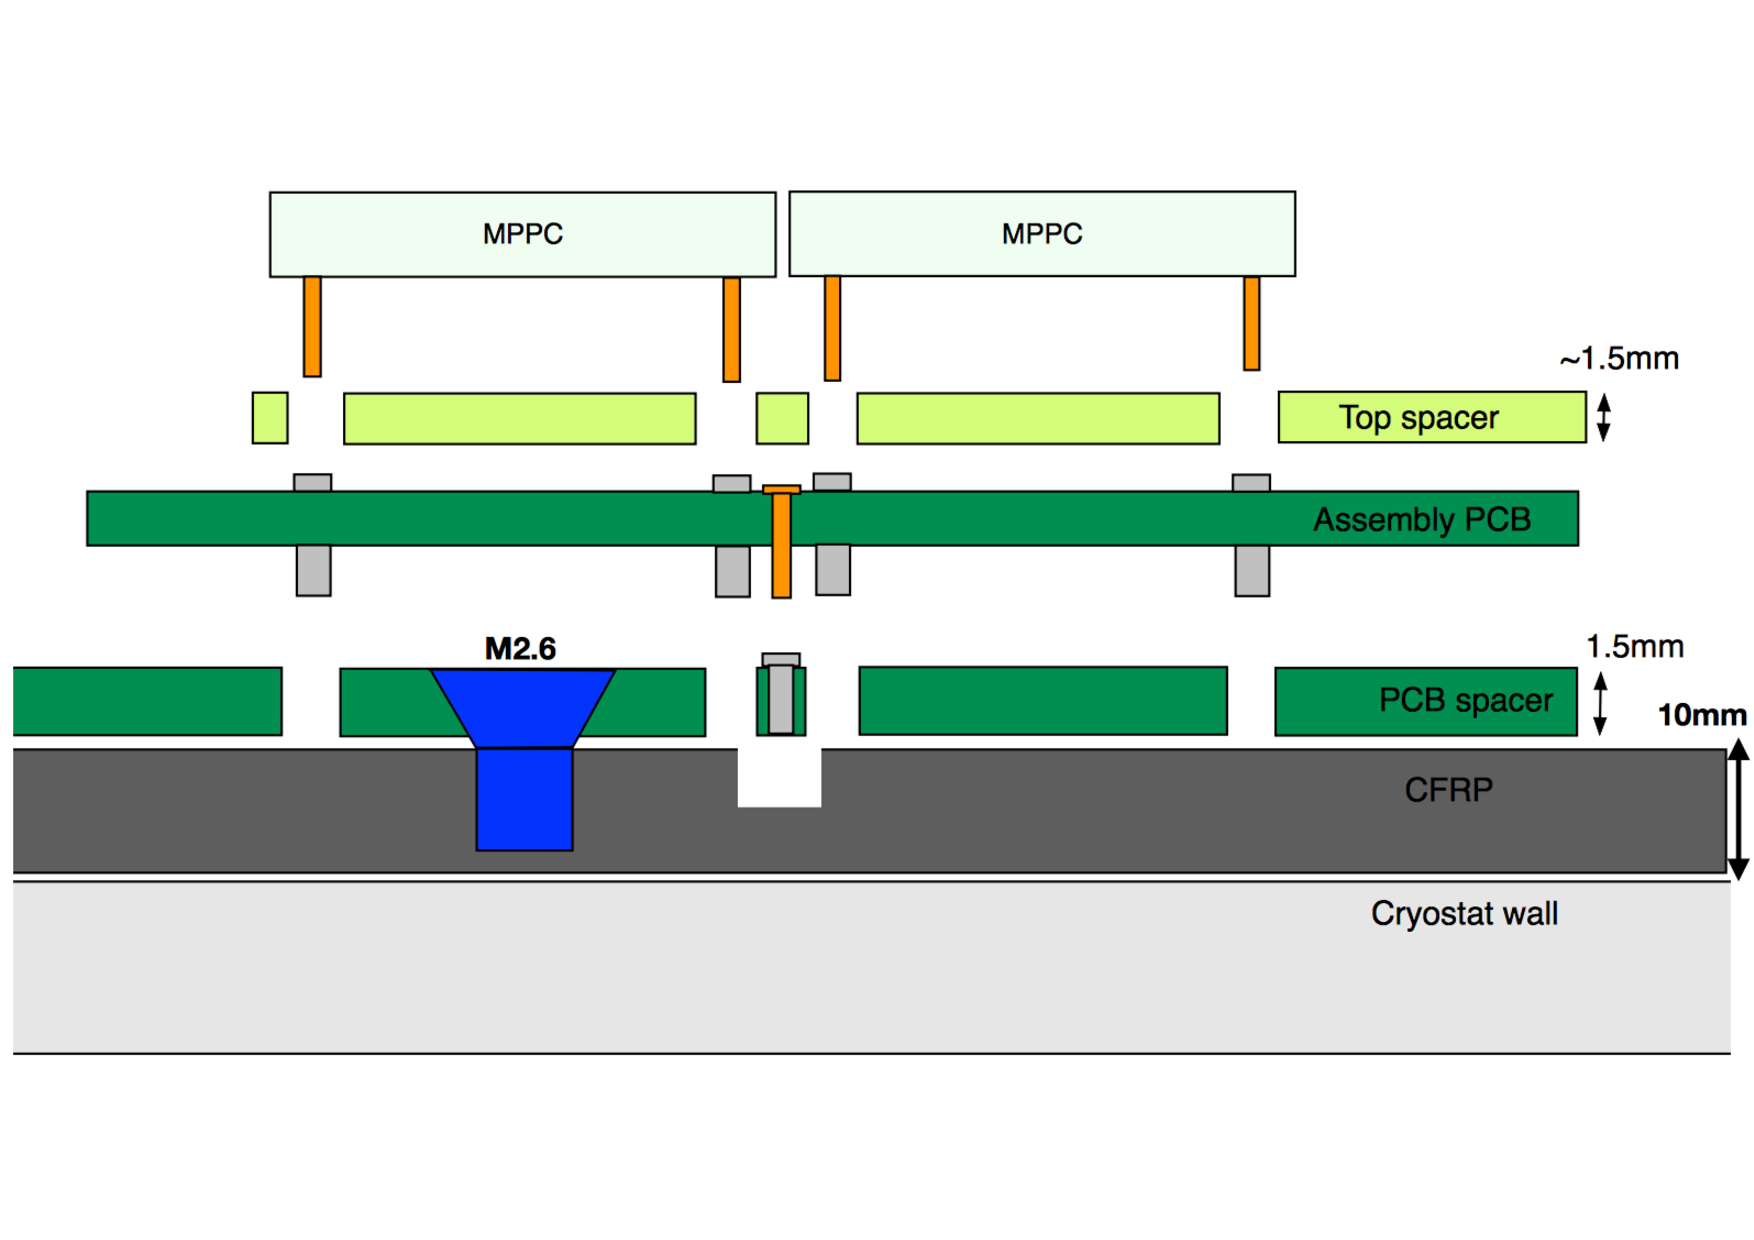
\includegraphics[width=4cm]{plots/MPPC_support.pdf}
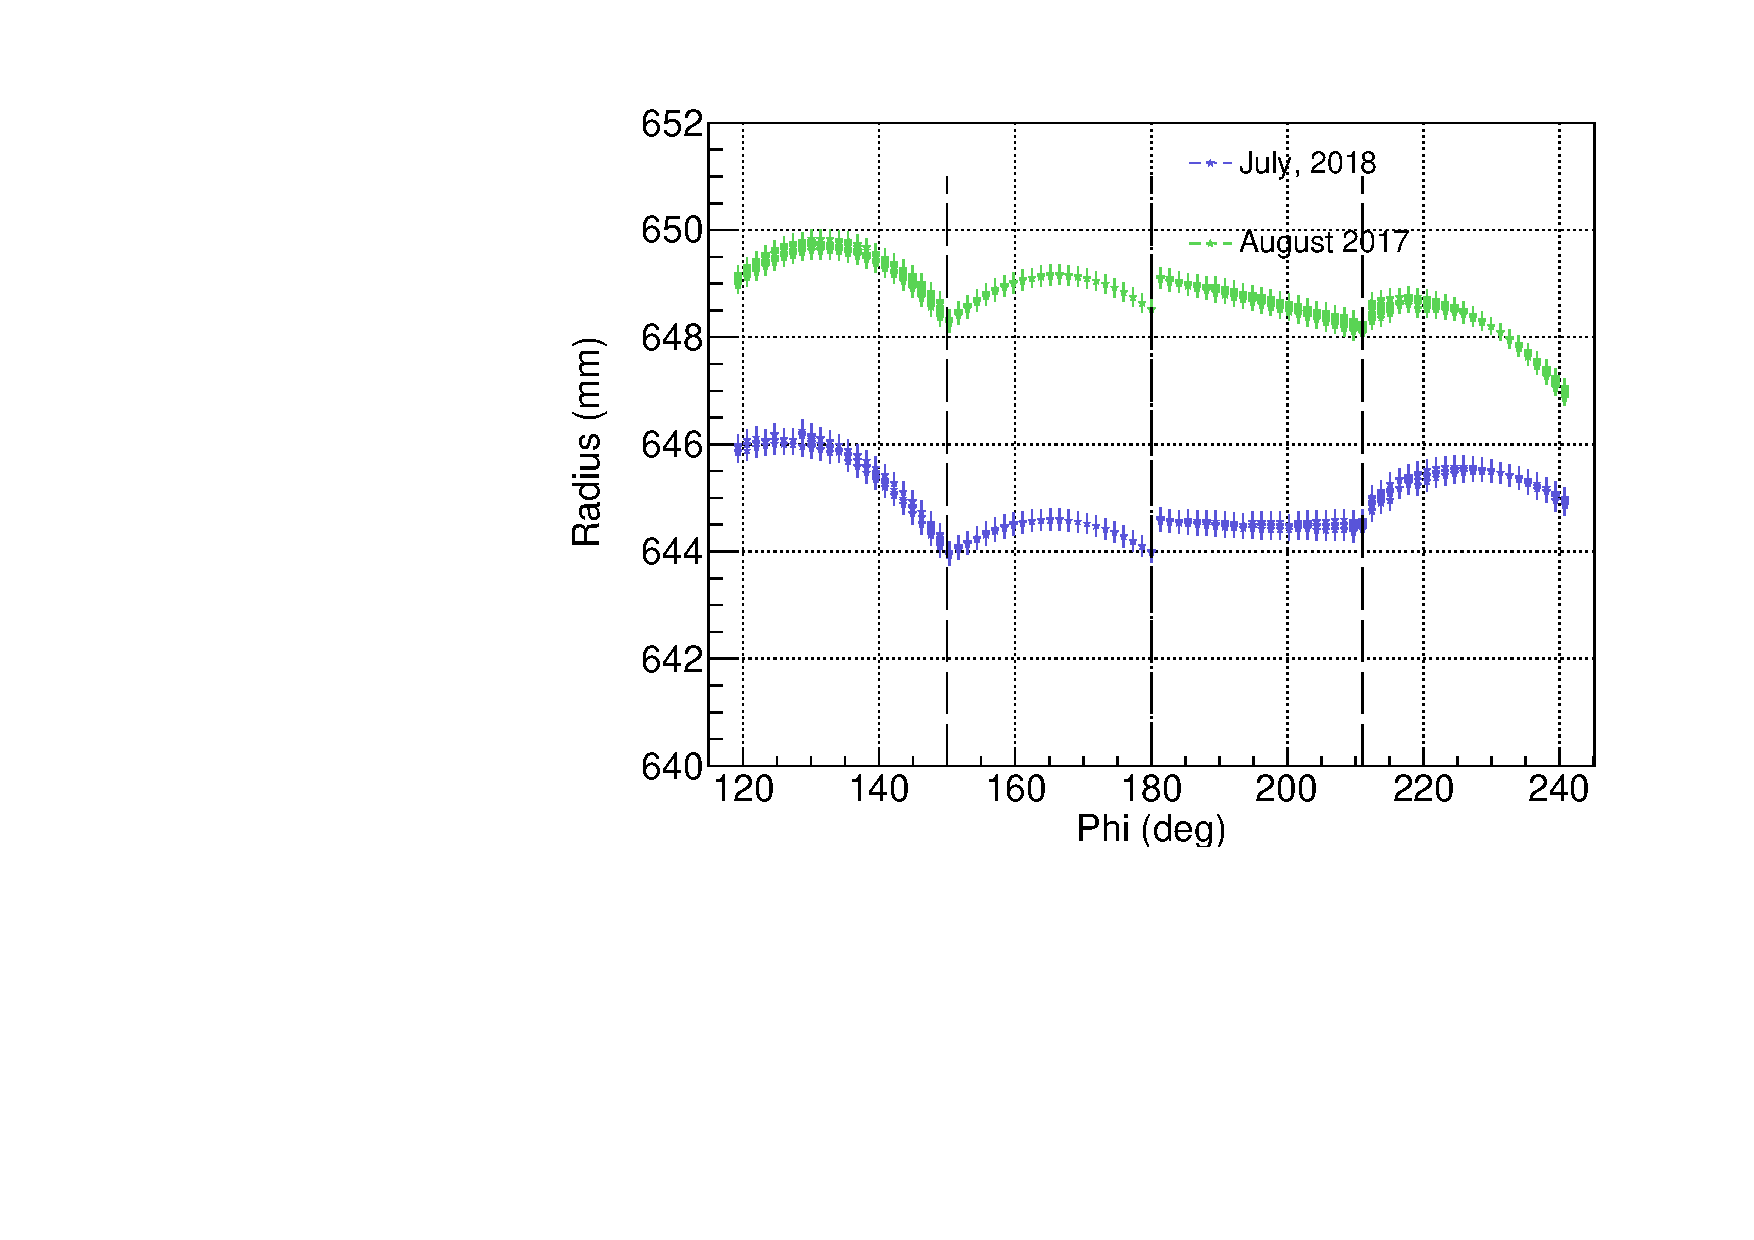
\includegraphics[width=4cm]{plots/2018/cRadius_1718}
\caption{ Radial coordinate of photodetectors with errors from 2017 and 2018
X-ray scans.  Black dashed lines indicate the edges of the CFRP board.}
\label{fig:radiuscalculation} 
\end{figure}



\noindent {\bf MPPC position, coeffient of thermal expansion  
            and X-ray interaction rate -- 2017 vs 2018} \\ 
The X-ray scans together with the fitted radial coordinate
provide a 3D location of each scanned photodetector  with high
precision ($\sigma_{|\vec{x}|}<0.5$~mm).  These measurements are
compared to a set of nominal positions in the designed detector
in order to reveal changes due to manufacturing and installation.
Secondly, the two X-ray  measurements are fitted to find global
offsets in the absolute positions which could be introduced due
to the movement of the calorimeter or thermal cycling of LXe
scintillator conducted between the two scans.

The nominal positions of the photodetectors
($Z_{MPPC}$, $\phi_{MPPC}$) are in a regular grid along
a cylindrical surface with constant radius, and its central
axis aligned with the Z axis of the MEG coordinate system.  
As shown already by the radial coordinate calculation
the photodetector placement is not perfectly uniform.
We find that the calorimeter can be divided into four separate
regions formed by the cfrp plates. Within each plate
there is rotation of the photodetectors about the radial
axis which causes $\phi$ dependent variation in the 
Z coordinate and corresponding and equal 
Z dependent variation in the $\phi$ coordinate
of the MPPC measured by the X-ray scan 
(figure \ref{fig:rotation}). The deviation of 
the measured from the 
nominal in Z and $\phi$ coordinates is fitted 
independently on mutiple subsets of photodetectors 
within each cfrp plate. The results (table \ref{tab:rotation})
show the mean slope due to the rotation varies between
2-5~mrad  or 1-4~mm dispalcement of the photodetector
over the entire calorimeter. The figures and the table 
show calculations using 2017 data, the results from 
the smaller 2018 data are found to be identical but not used.
\\
\\
\\

\noindent 2d plots in xy plane \\
Check for deformation based on Comparison to faro measurement - dry vs wet detector.\\
--Thermal contraction, fitted position values\\

\begin{table}
\begin{tabular}{ccc}
   & $dZ/d\phi_{MPPC}$ & $d\phi/dZ_{MPPC}$ \\
\hline 
cfrp 1 & -0.0025 & 0.0033 \\
cfrp 2 & -0.0032 & 0.0040 \\
cfrp 3 & -0.0033 & 0.0045 \\
cfrp 4 & -0.0050 & 0.0058 \\
\end{tabular}
\caption{Average slopes (mm/mm) of deviation between X-ray and nominal MPPC positions
$dZ, d\phi$ with respect to the other coordinate, shown for each 
cfrp plate.
}
\label{tab:rotation}
\end{table}

\begin{figure}
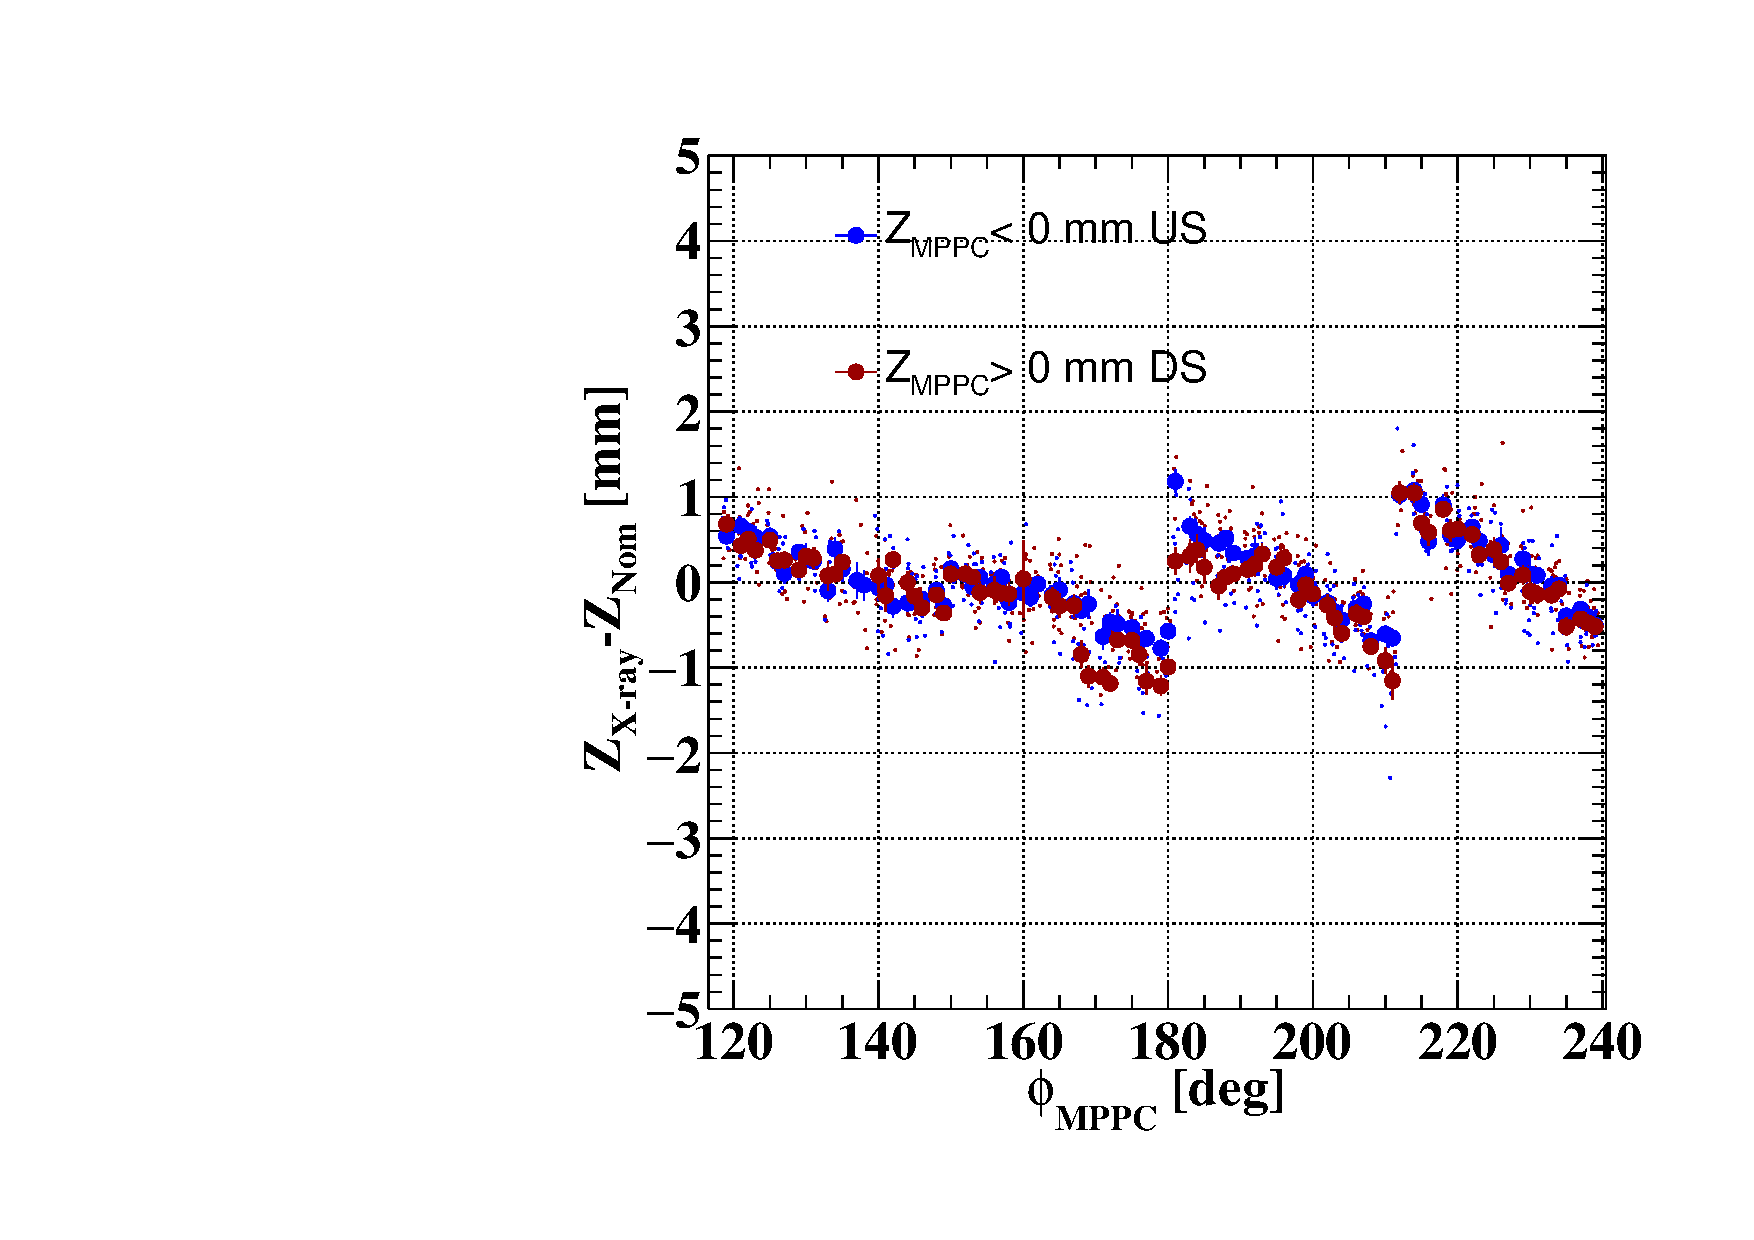
\includegraphics[width=4cm]{plots/dz_boardrotation.pdf}
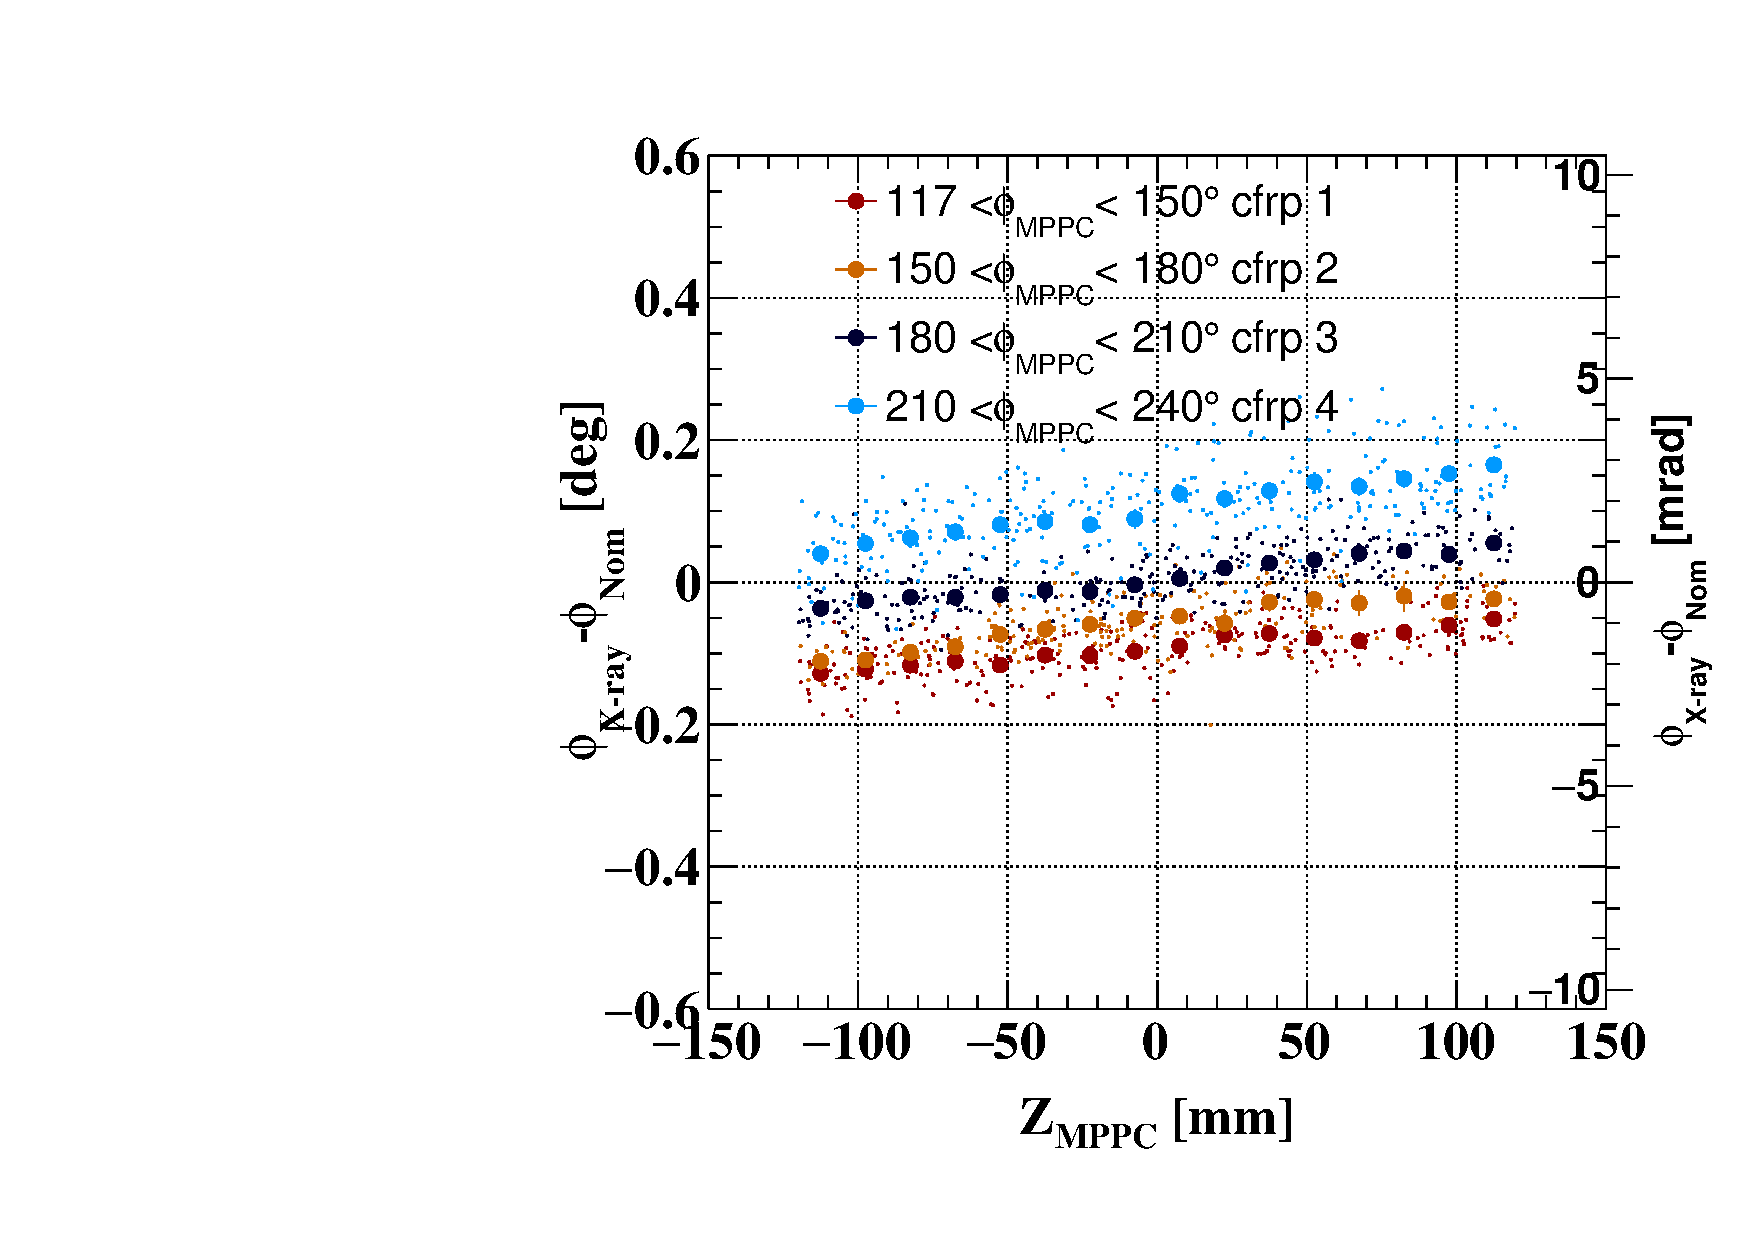
\includegraphics[width=4cm]{plots/dphi_boardrotation.pdf}\\
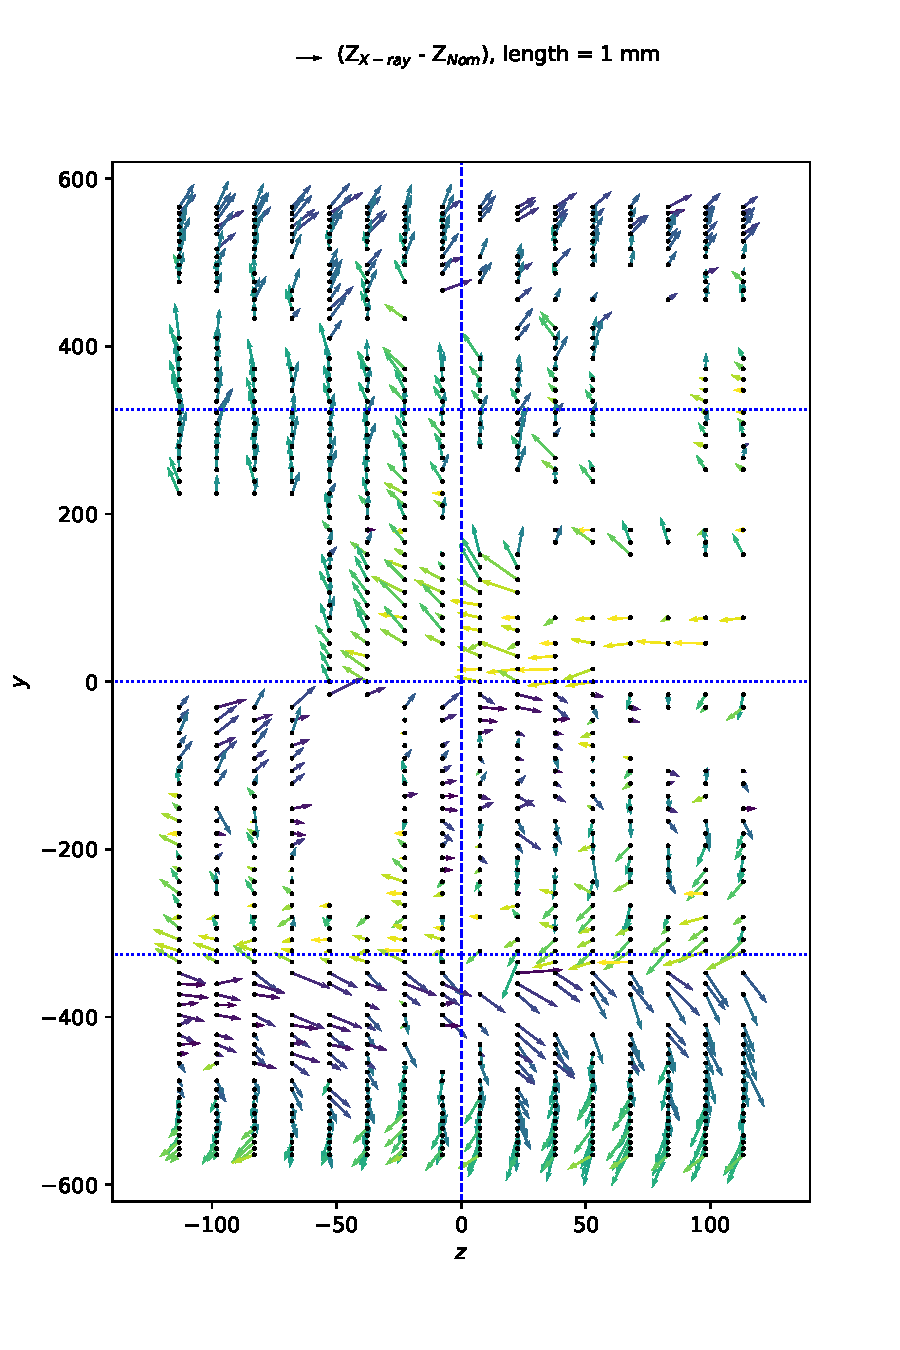
\includegraphics[width=8.5cm]{plots/dzdy2017_rx.pdf}
\caption{[add cfrp boundary]
Difference between the X-ray measured and nominal MPPC positions
overlayed with the profile histogram (scatter plots).
US and DS PCB half-strips and cfrp plates are shown separately.
Arrow plot showing rotation of the MPPCs with respect to nominal
positions in the YZ plane; dotted horizontal lines show cfrp plate boundaries,
dashed vertical line at the center separates the PCB half-strips (arrow plot).
Both Z and $\phi$ measurements have global offsets with respect to the 
nominal which are corrected in the plots.
}
\label{fig:rotation}
\end{figure}


The efficacy of spacer materials between MPPC, PCB strip and CFRP
board is tested by examining the X-ray event rate as a function of
MPPC position. The rate is inversely proportional to the length of LXe
traversed by the X-ray before interaction.  It provides crucial
information about the state of spacer materials responsible for
preventing LXe leak between inner cryostat wall and the photosensitive
surface, which directly impacts photo detection and reconstruction
efficiencies, and energy response.  A constant rate of triggered
events is expected from all scanned MPPCs with some variation
attributed to electronic readouts that are nominally configured in an
identical way.  The event rates show a $\phi$ dependent variation
indicating some deformation in CFRP boards 1 and 2.  A drop in the
rates by a factor 1/e suggests the scale of deformation
$\approx\,\lambda_{\mathrm{Xe}}$.  The $\phi$ dependent variation is
observed in both Z and $\phi$ scans in the MPPCs illuminated with
X-rays and is not seen in the background process
(Figure~\ref{fig:ratesvszphi}).  The second scan in 2018 replicates
the previous years data at a lower rate due to reduced activity of the
source by two half-lives.  \begin{figure}[]
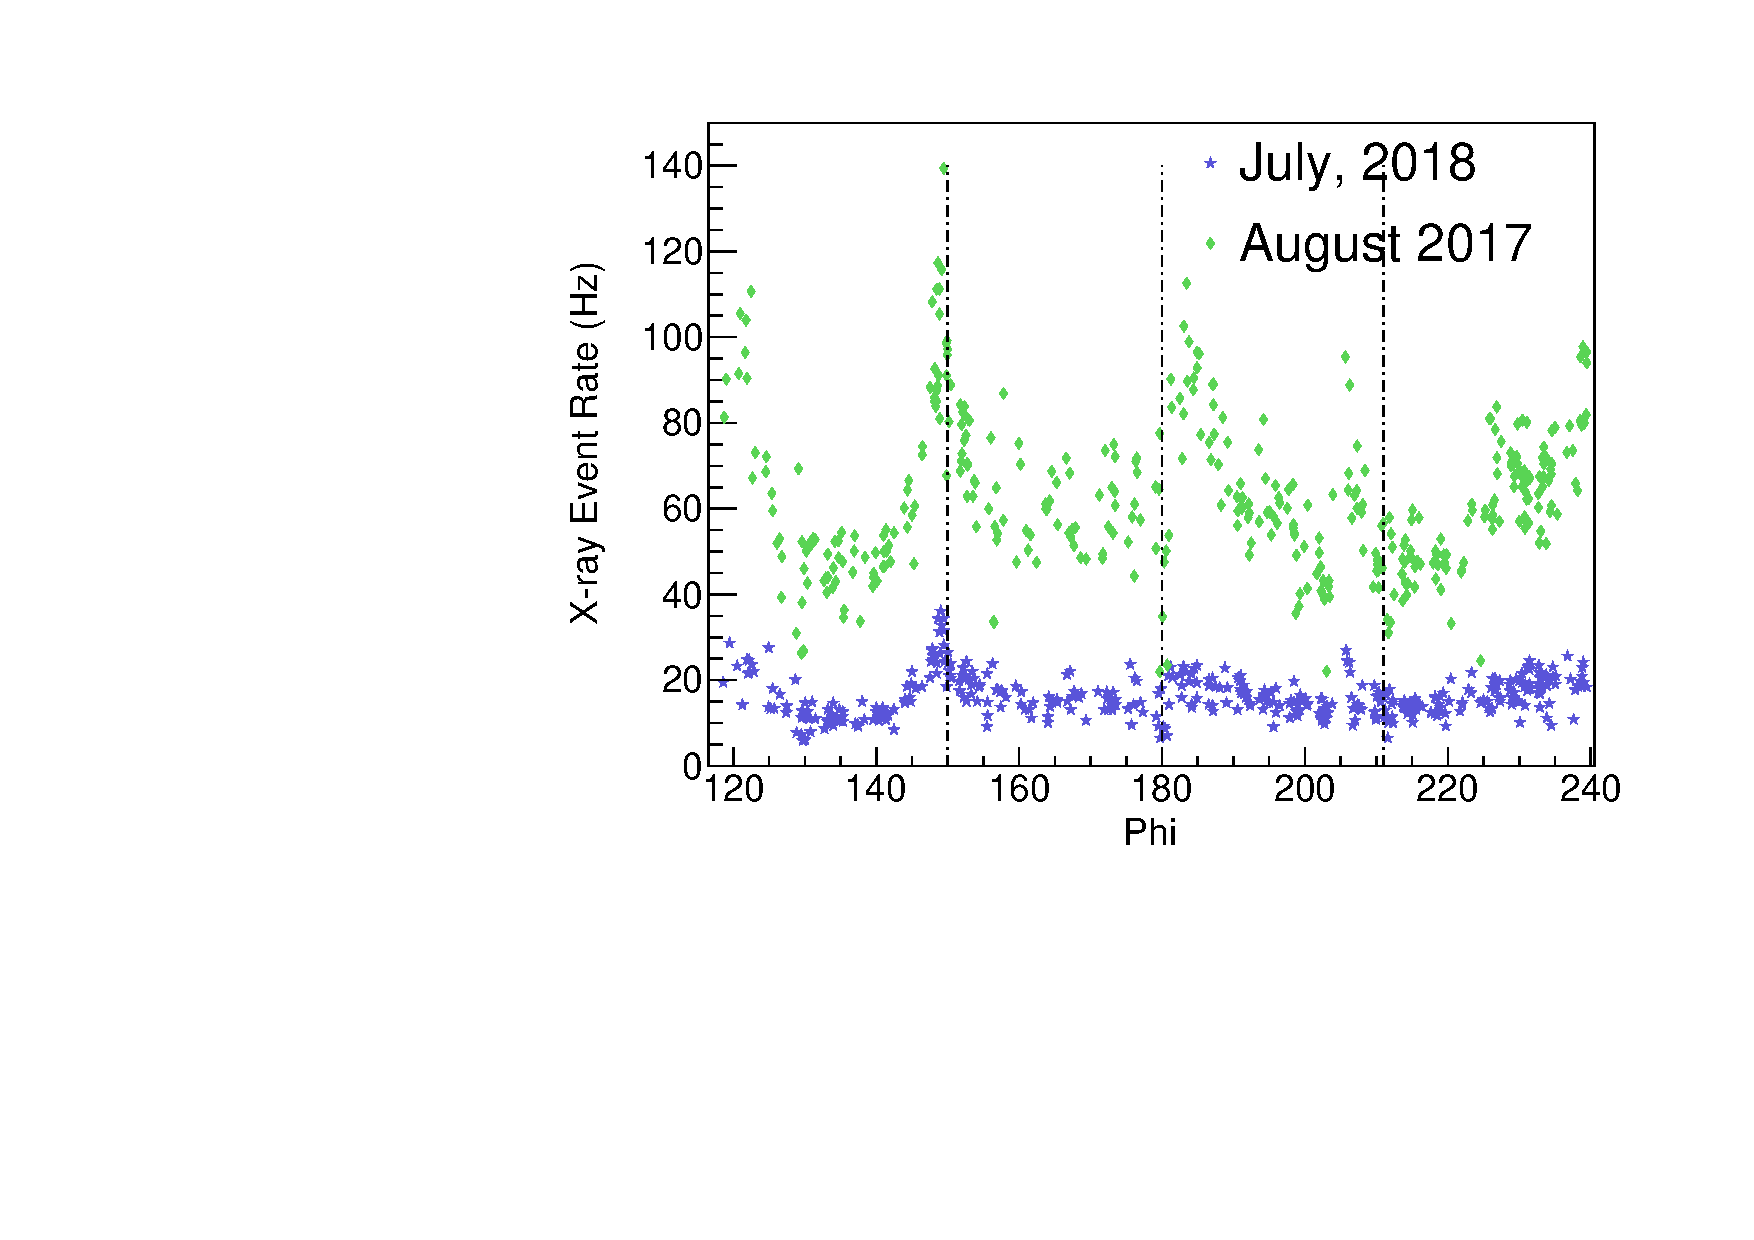
\includegraphics[width=4cm]{plots/2018/cEventRate_1718}
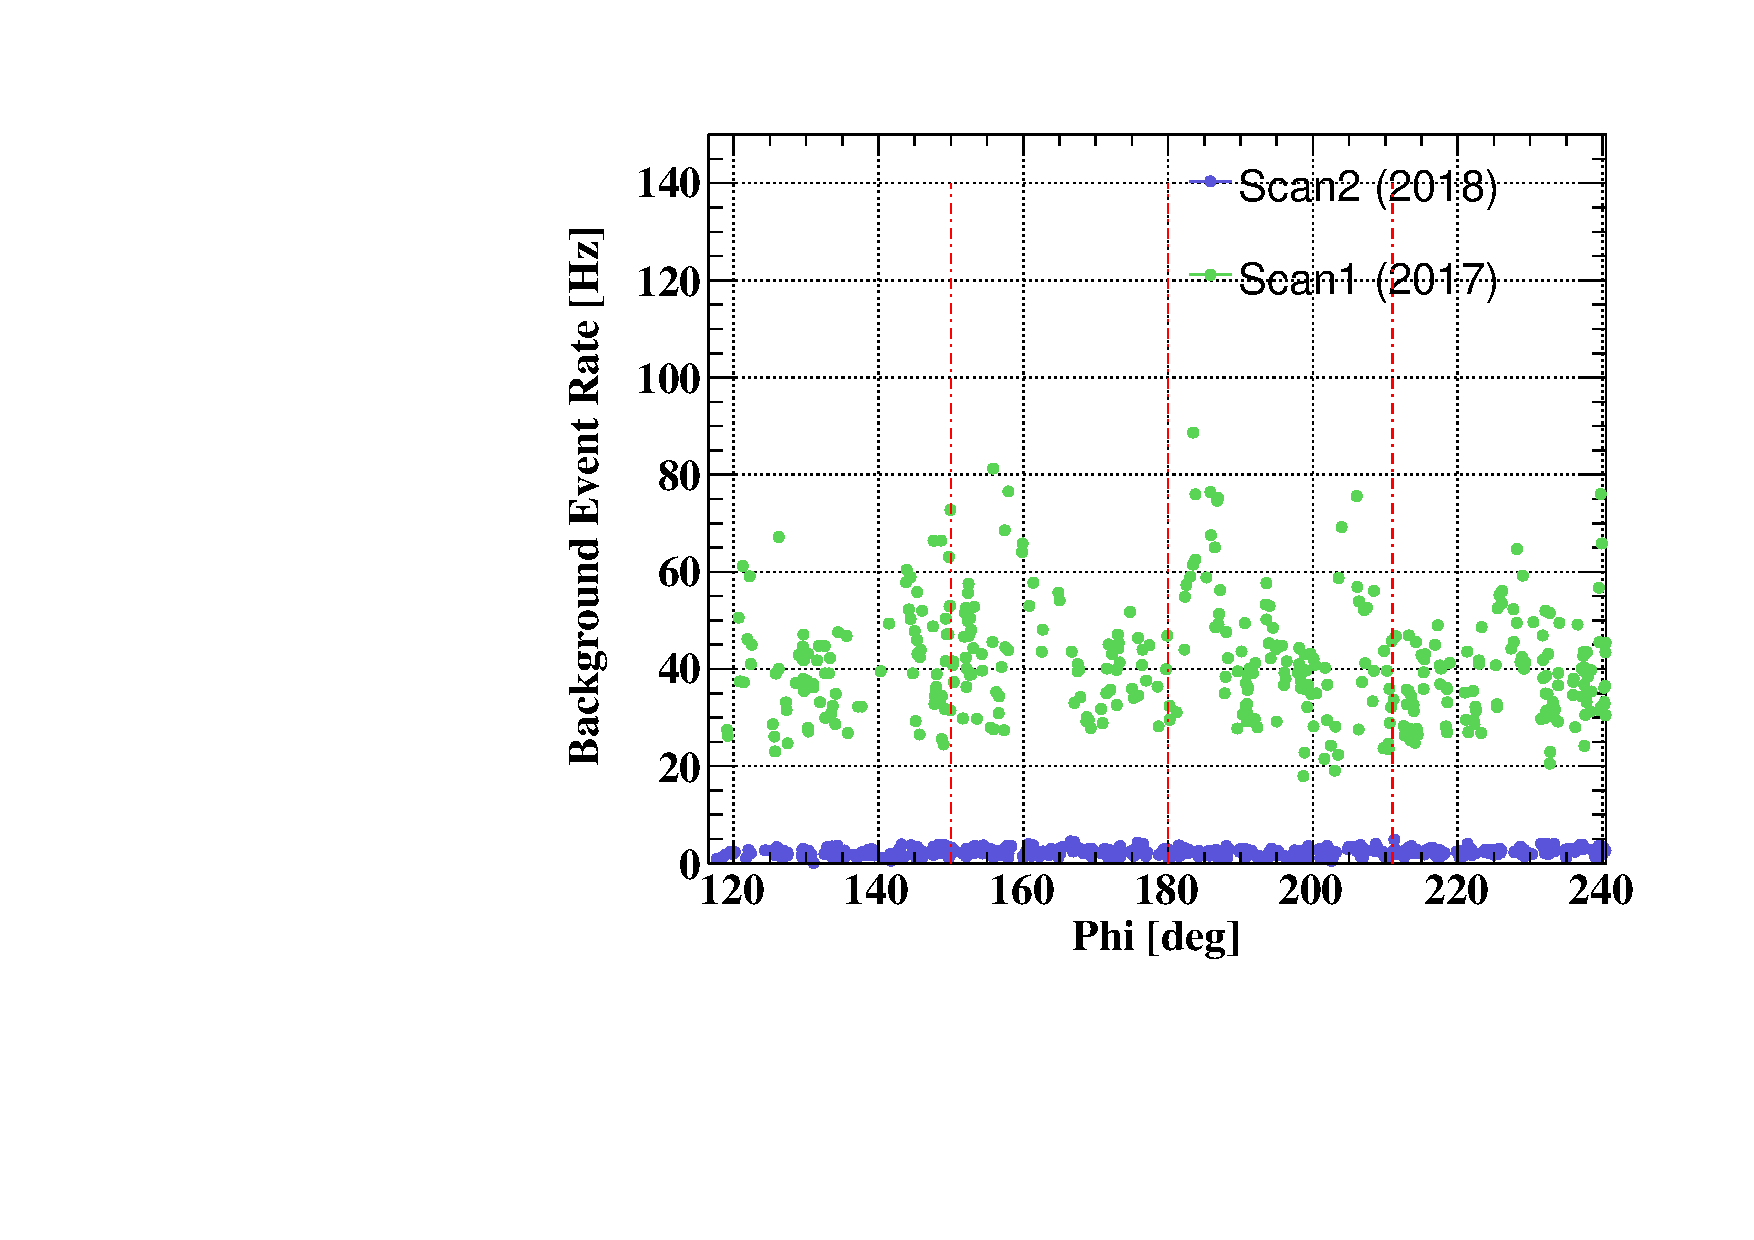
\includegraphics[width=4cm]{plots/2018/cBkgRate_1718} \caption{Signal
and background trigger rates observed in MPPC as a function of $\phi$.
Black lines indicate the edges of the CFRP board.}
\label{fig:ratesvszphi} \end{figure}





\subsection{Secondary Checks On Photodetector Fit Positions}
Given that there are certain levels of variance in the exact shape of the photodetector outlines, produced in the rate plots, we will ensure that any fitting that has been done to find central values is stable -- across repeated fitting -- and repeatable across multiple measurements.

To ensure the stability of our fitting methodology, two separate analyses were done on all the same data runs (excluding the lead-strip based data) with all steps being identical -- as described in Sec. \ref{mppcposition} -- except that the central point is determined using different choices of fitting function; the first fit choice is to be a piece-wise construction (Eqn. \ref{eqn:linetwogaus}) whereas the second is an eighth power supergaussian (Eqn. \ref{eqn:supergaus}). Hence, we can do a detailed comparison of how strong the agreement is between the found centers for all photodetectors which are well fit by both functions.

In Fig. \ref{fig:difffits} and Table \ref{tab:fitfcndiff}, there is good agreement between fit functions in both coordinate axes, as even the larger of the mean differences -- $212\, \mu rad \, \sim\, 138\, \mu m$, with $\sigma_{RMS} \, \sim \, 281 \, \mu m$ \footnote{Conversions done with radius approximated to 650mm} -- is still well within expected levels of uncertainty inherent to the forms of measurement used by this study. 
\begin{figure}[H]
    \centering
    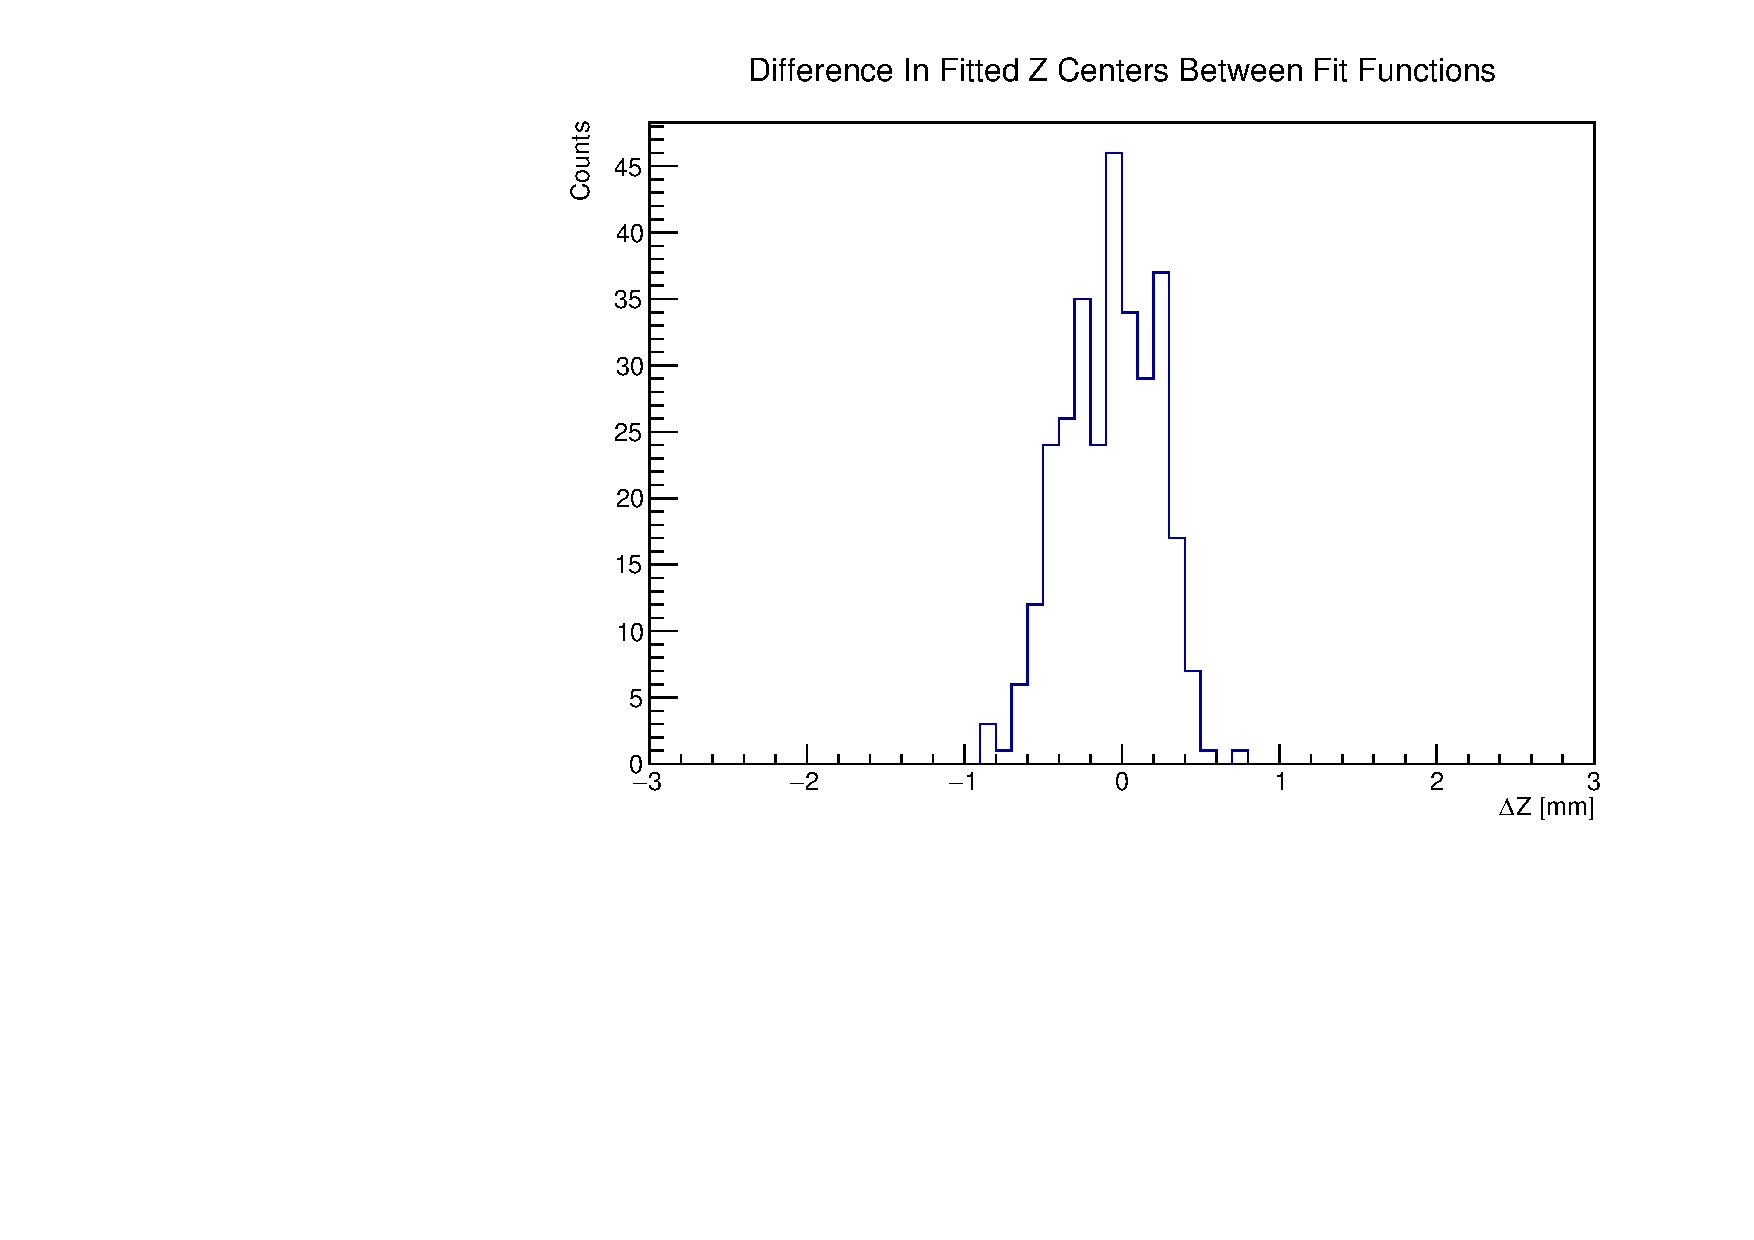
\includegraphics[width=4.25cm]{graphics/terdzns.pdf}
    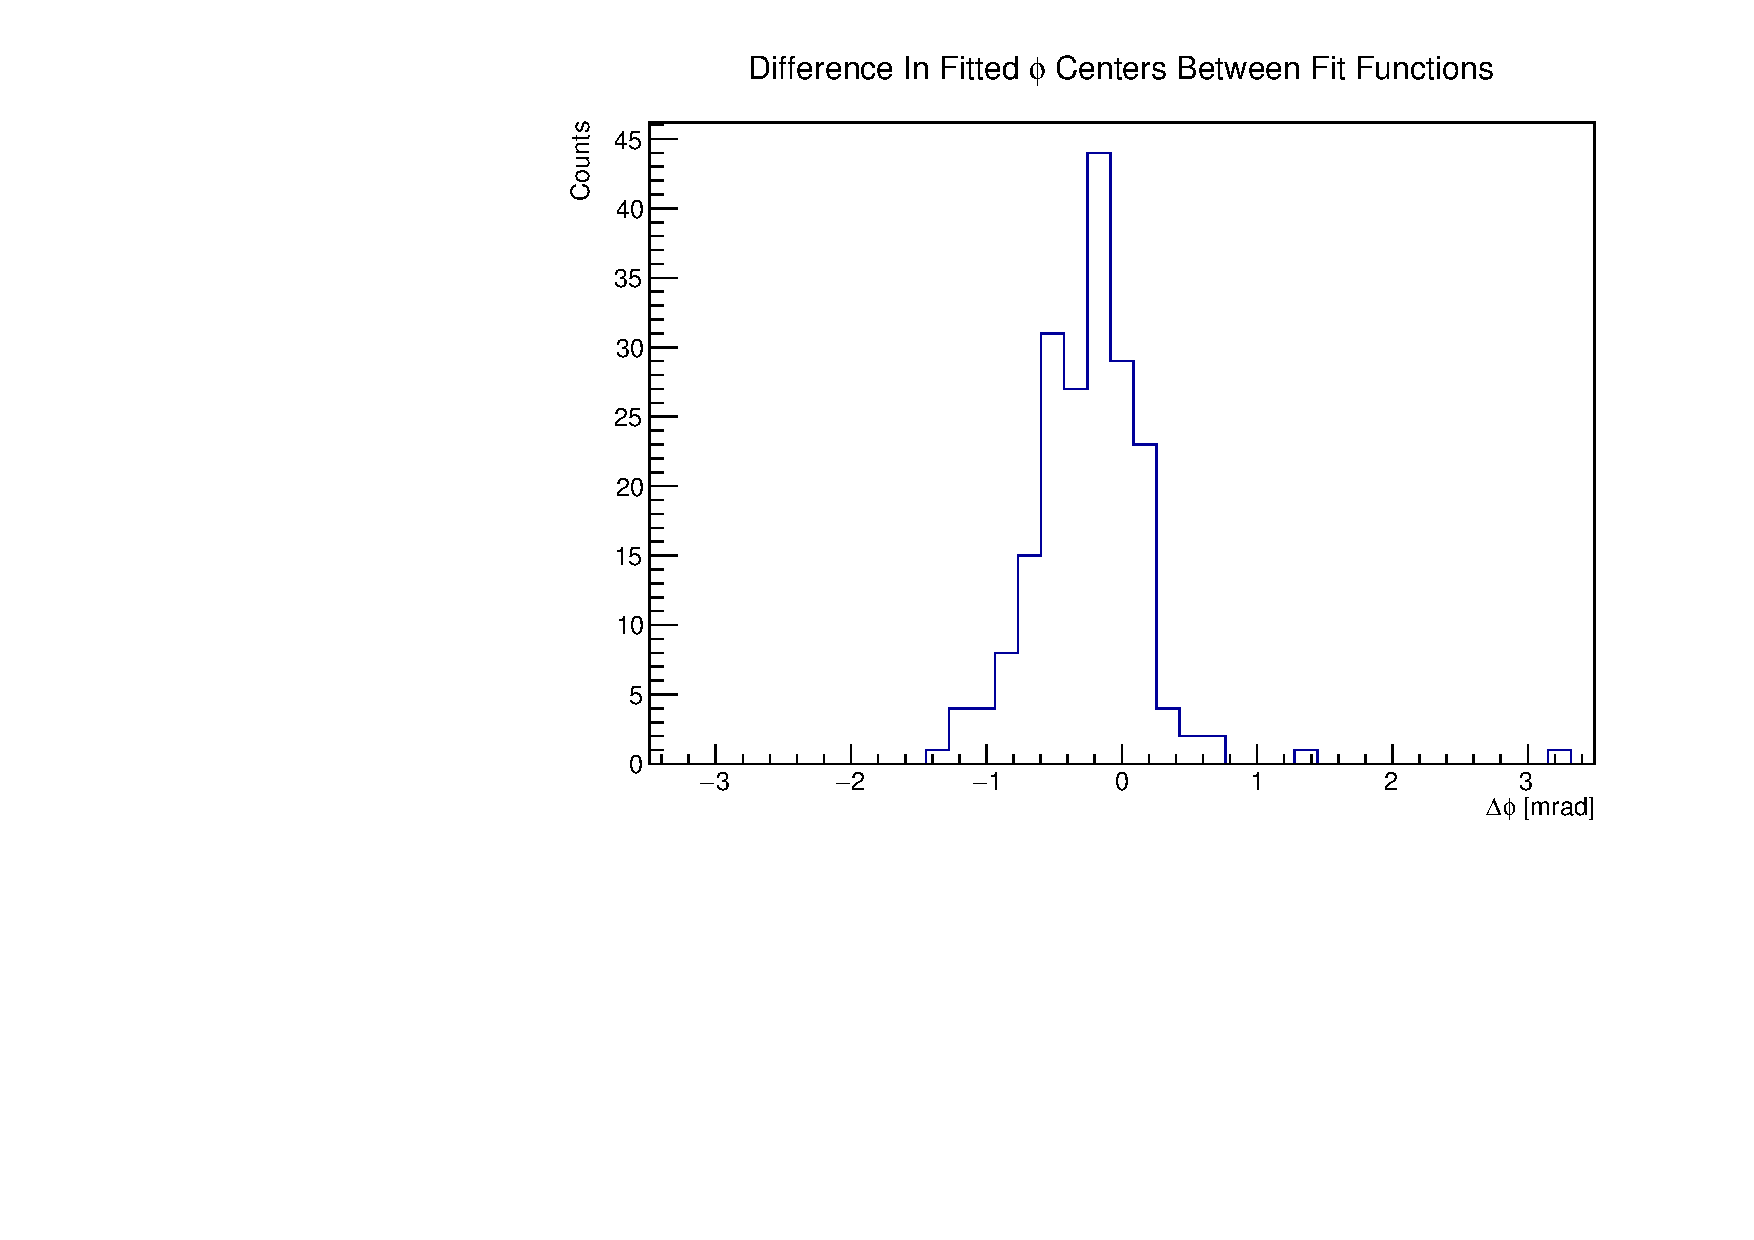
\includegraphics[width=4.25cm]{graphics/terdpns.pdf}
    \caption{Histogram Of Difference In Found Centers For All Z Scans (left) And All $\phi$ Scans (right) For Differing Fit Functions}
    \label{fig:difffits}
\end{figure}

\begin{table}[H]
    \centering
    \begin{tabular}{c c|c c}
        $\mu_{dZ}$ [mm]& $\sigma_{RMS}$ [mm]& $\mu_{d\phi}$ [mrad]& $\sigma_{RMS}$ [mrad]\\
        \hline 
        -0.0748 & 0.290 & -0.243 & 0.453 \\ 
         & & $\sim\,$-0.157 mm & $\sim\,$0.292 mm 
    \end{tabular}
    \caption{Average Disagreement Of Centers In Using Alternate Fit Functions}
    \label{tab:fitfcndiff}
\end{table}

%%\begin{comment}
%%\begin{table}[H]
%%    \centering
%%    \begin{tabular}{c|c||c|c}
%%        $\mu_{dZ}$ [mm]& $\sigma_{RMS}$ [mm]& $\mu_{d\phi}$ [mrad]& $\sigma_{RMS}$ [mrad]\\
%%        \hline
%%        -0.1281 & 0.2323 & -0.2119 & 0.4333
%%    \end{tabular}
%%    \begin{tabular}{c c||c|c}
%%         & & $\mu_{d\phi}$ [mrad]& $\sigma_{RMS}$ [mrad]\\
%%        \hline
%%         & & -0.2119 & 0.4333
%%    \end{tabular}
%%    \caption{Average Disagreement Of Centers In Using Alternate Fit Functions}
%%    \label{tab:fitfcndiff}
%%\end{table}
%%
%%\end{comment}

To check the repeatability of this measurement technique, there were 14 well-fit photodetectors which were scanned more than once in the same physical (Z-scan) setup. In  Fig. \ref{fig:repzmeas} and Table \ref{tab:mulitscandz}, a comparison is shown between these measurements taken in different scans.
\begin{figure}[H]
    \centering
    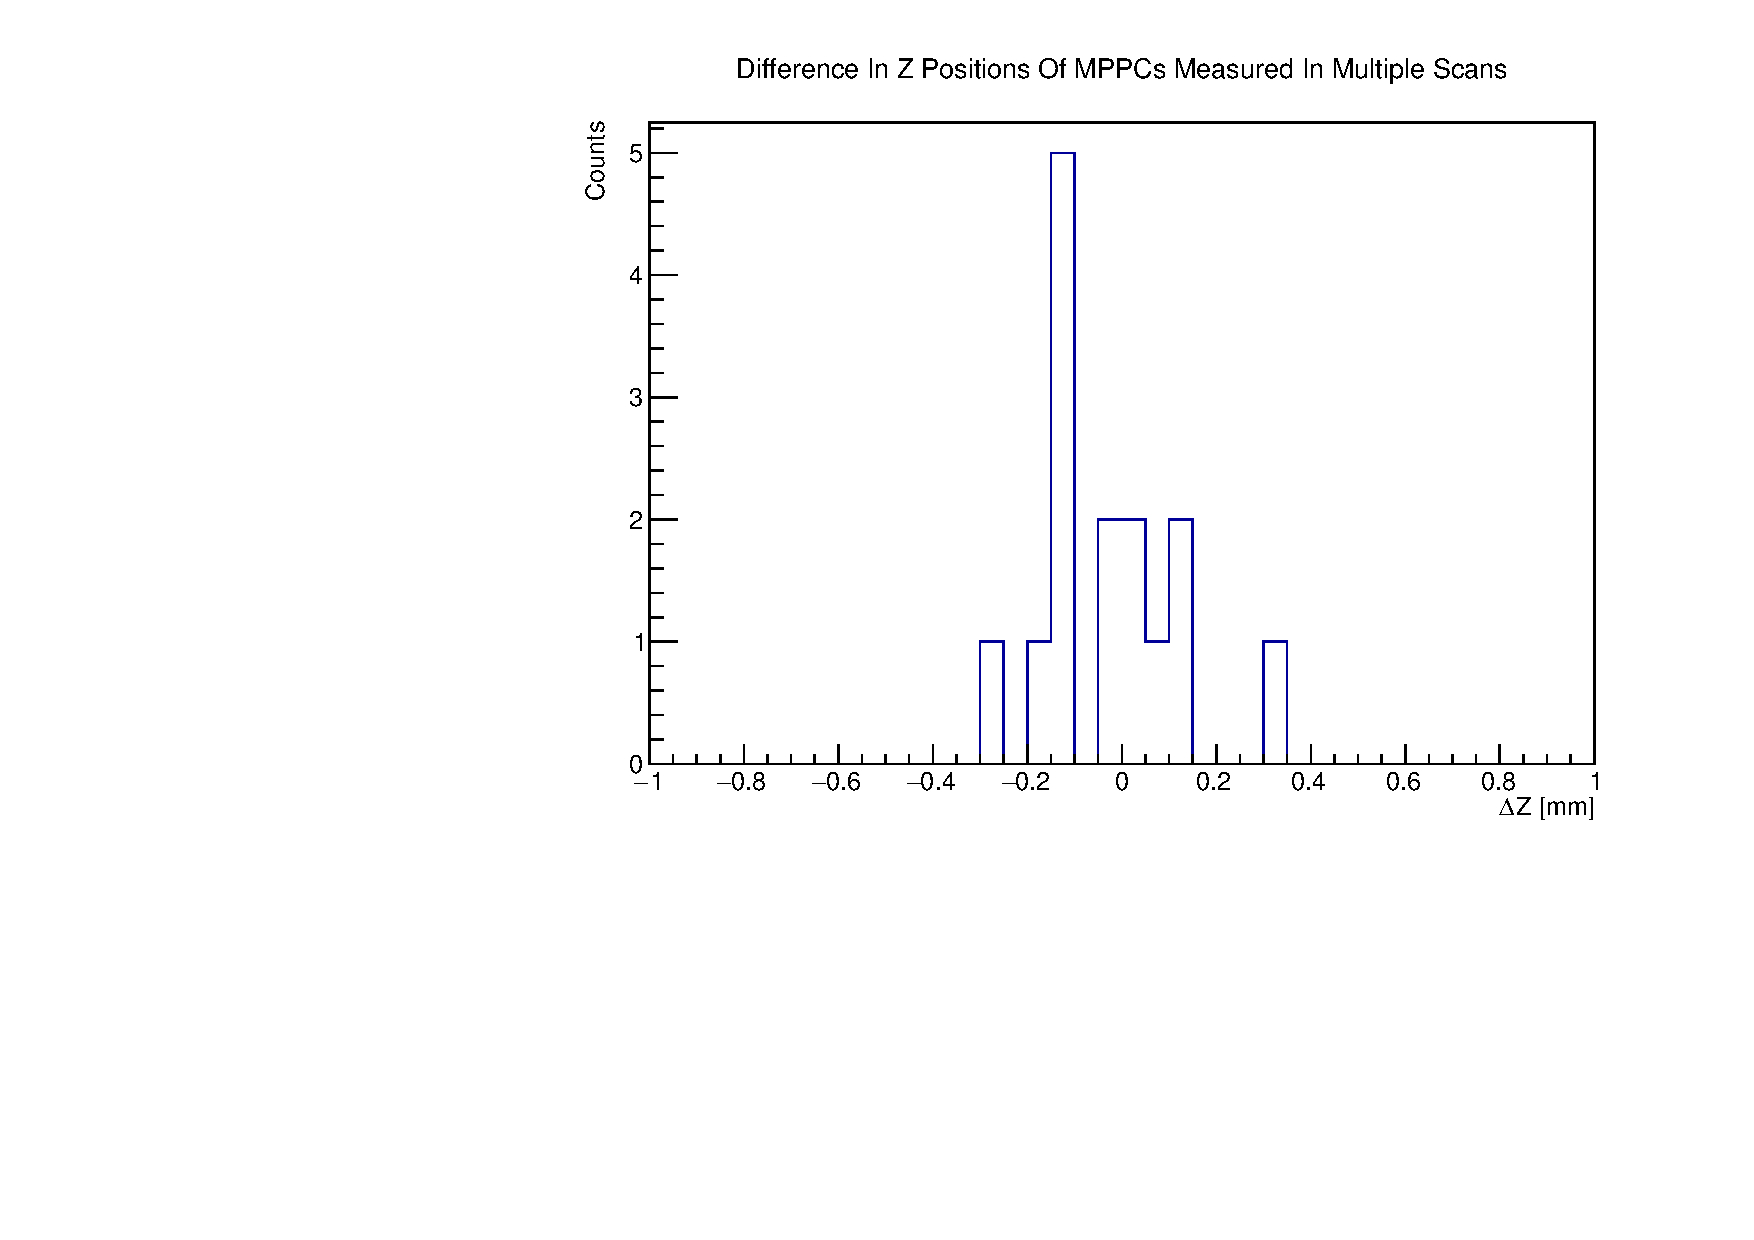
\includegraphics[width=6cm]{graphics/repdzbnostats.pdf}
    \caption{Comparing Centers From Repeated Detector Scans}
    \label{fig:repzmeas}
\end{figure}
\begin{table}[H]
    \centering
    \begin{tabular}{c|c}
        $\mu_{dZ}$ [mm]& $\sigma_{RMS}$ [mm]  \\
        \hline
        -0.03271 & 0.1466
    \end{tabular}
    \caption{Average Disagreement In Supergaussian Fit Centers For Multiple Scans Of The Same Photodetector}
    \label{tab:mulitscandz}
\end{table}
\noindent 
So again, we find the level of disagreement shown above is still well within expected levels of uncertainty.

\subsection{Charge Asymmetry} \label{chargeasym}
\noindent An additional measurement of each photodetector's edge location was determined by fitting charge asymmetries (Eqn. \ref{qasymeqn}) between adjacent photodetectors. 
This allows for a determination of photodetector edges as defined by the midpoint between two detectors, where the X-ray beam induces equal charge measurements.
\begin{equation} \label{qasymeqn}
    \mathrm{Asymmetry[Z_{n}] = \frac{Charge[Z_{n},\phi_{m}]-Charge[Z_{n+1},\phi_{m}]}{Charge[Z_{n},\phi_{m}]+Charge[Z_{n+1},\phi_{m}]}}
\end{equation}
To select the proper X-ray events, a nearly identical set of criteria to those from Sec. \ref{mppcposition} was used:
\begin{enumerate}
    \item A sum of the charges in the asymmetry's two photodetectors is required to be both relatively and absolutely large ($> 70\%,\,>0.4$ pC).
    \item Every individual photodetector in the negative trigger region (measuring background signal) is required to be small ($< 0.1$ pC).
\end{enumerate}
 These plots were then fit to the following functional form,
\begin{equation}
    \mathrm{Asymmetry\; Fit \,}(x)=\;\mathrm{A}\,\left[\,\mathrm{Erfc}\left(\alpha(x-x_{0})\right)-1\,\right]
\end{equation}
and one example of this procedure is displayed in Fig. \ref{fig:asymexample}.
\begin{figure}[H]
\centering
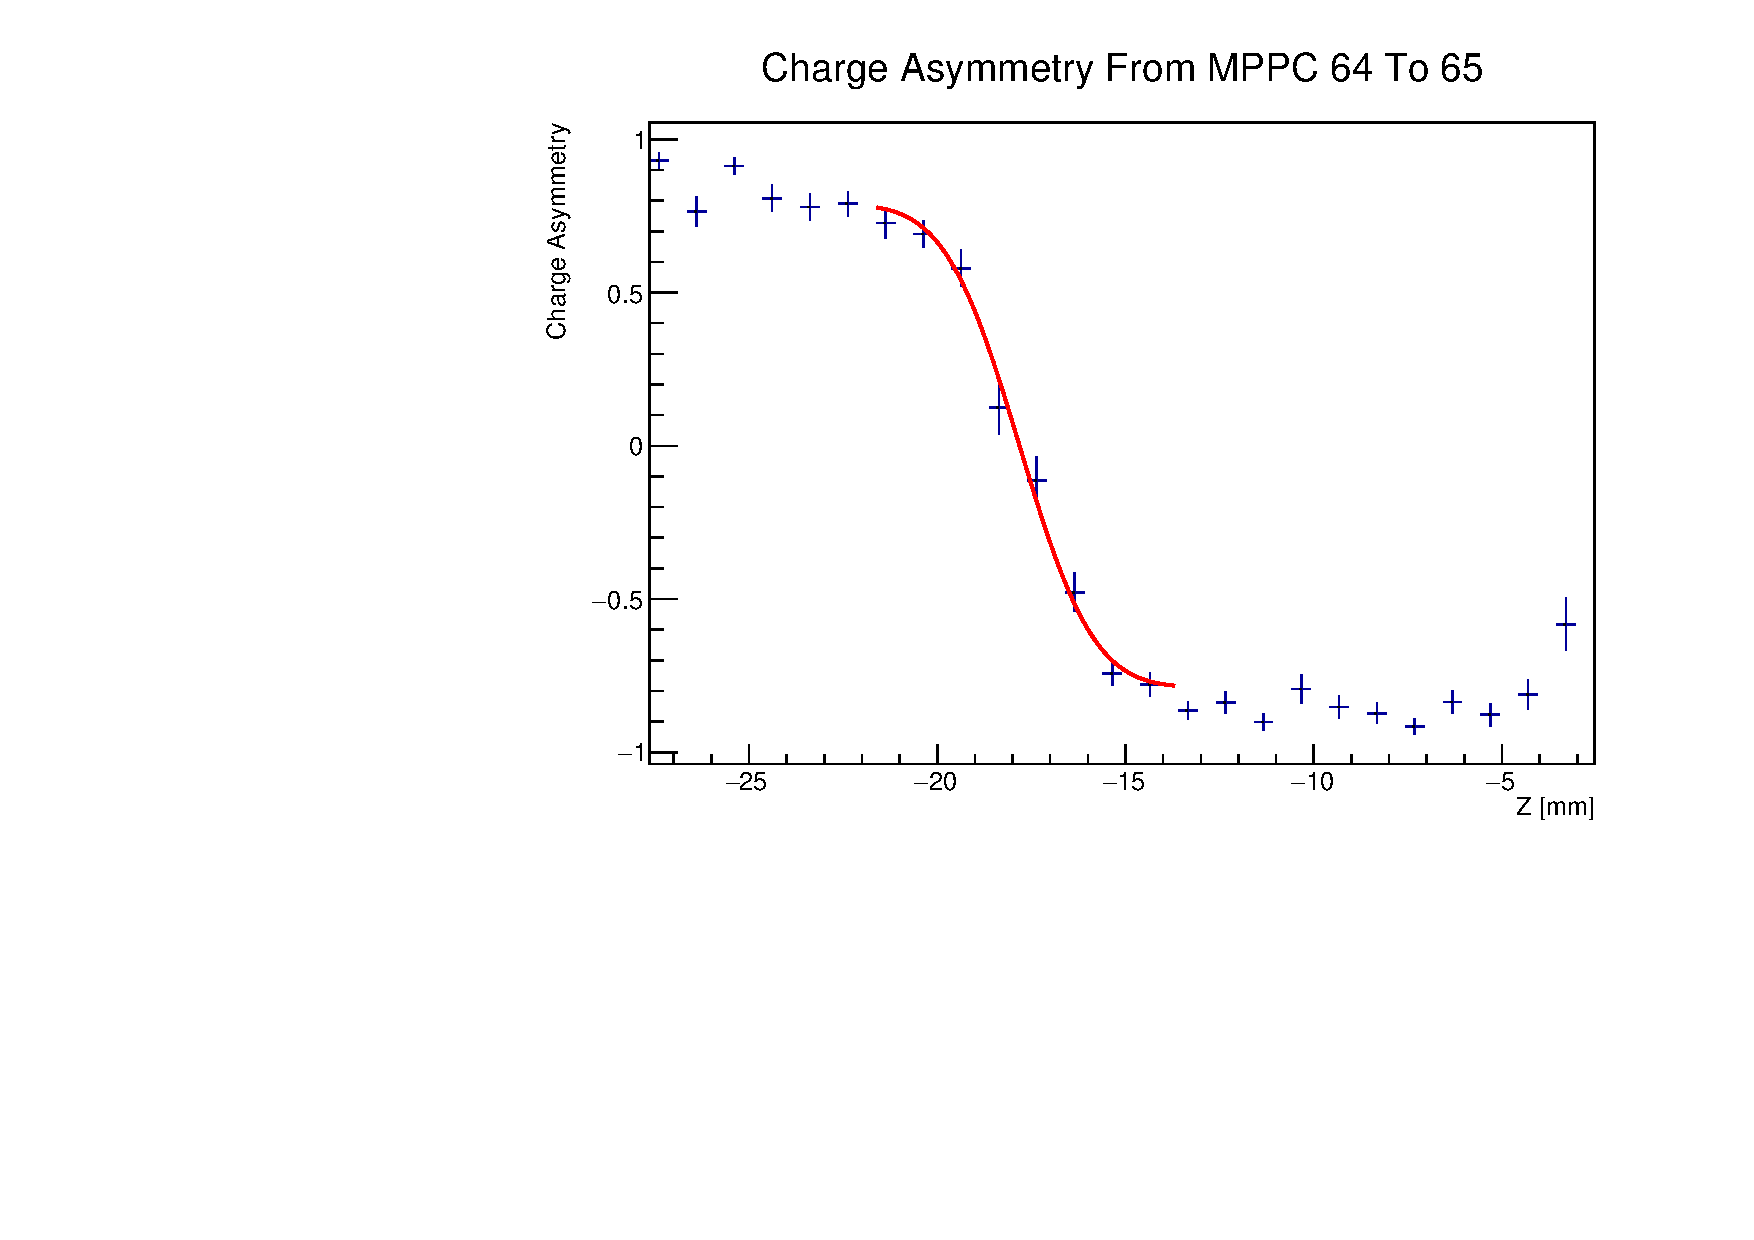
\includegraphics[width=7cm]{graphics/asym6465.pdf}\caption{
Calculated Charge Asymmetry With Fit}
\label{fig:asymexample} 
\end{figure}

Importantly, we gain normalized all the photodetectors to the same response magnitudes, thereby removing any artificial shift in the zero-point of our asymmetries. This was done through averaging the charge from all events within 6mm of the previously fitted centers of each MPPC, and subsequently dividing the necessary charge measurements by these averages.


With these additional measurements, it is possible to produce a comparison to our prior findings on the photodetector spacing. For this purpose, we calculate all the possible offsets of detectors edges (per asymmetry fits) from their previously fitted central locations. 
\begin{table}[H]
    \centering
    \begin{tabular}{c||c|c}
        \bf Upper Edge & \bf \boldmath$\mu$ [mm] & \bf \boldmath$\sigma_{RMS}$ [mm] \\
         \hline
        Even, 1 of 4 & 7.954 & 0.500 \\
        Even, 3 of 4 & 7.824 & 0.409 \\
        Even, 1 of 2 & 7.82 & 0.438  \\
        Odd, 2 of 4 & 7.713 & 0.396  \\
        \hline
        All Even & 7.862 & 0.451 \\
        All Odd & 7.713 & 0.396
    \end{tabular}
    \caption{Measured Z Offsets of Upper Edges From Fit Centers}
    \label{tab:upperedgeasymz}
\end{table}
\begin{table}[H]
    \centering
    \begin{tabular}{c||c|c}
         \bf Lower Edge & \bf \boldmath$\mu$ [mm] & \bf \boldmath$\sigma_{RMS}$ [mm] \\
         \hline
         Odd, 2 of 4 & 7.363 & 0.385 \\
         Odd, 4 of 4 & 7.771 & 0.413 \\
         Odd, 2 of 2 & 7.816 & 0.410 \\
         Even, 3 of 4 & 7.154 & 0.436 \\
         \hline 
         All Even & 7.154 & 0.436 \\
         All Odd & 7.669 & 0.448
    \end{tabular}
    \caption{Measured Z Offsets of Lower Edges From Fit Centers}
    \label{tab:loweredgeasymz}
\end{table}

\begin{table}[H]
    \centering
    \begin{tabular}{c||c|c}
        \bf Upper Edge & \bf \boldmath$\mu$ [mrad] & \bf \boldmath$\sigma_{RMS}$ [mrad] \\
         \hline
        Even, 1 of 4 & 12.05 & 1.023 \\
        Even, 3 of 4 & 12.56 & 0.7336 \\
        Even, 1 of 2 & 12.28 & 0.357  \\
        Odd, 2 of 4 & 12.23 & 1.125  \\
        \hline
        All Even & 12.32 & 0.884 \\
        All Odd & 12.23 & 1.125
    \end{tabular}
    \caption{Measured $\phi$ Offsets of Upper Edges From Fit Centers}
    \label{tab:upperedgeasymphi}
\end{table}
\begin{table}[H]
    \centering
    \begin{tabular}{c||c|c}
         \bf Lower Edge & \bf \boldmath$\mu$ [mrad] & \bf \boldmath$\sigma_{RMS}$ [mrad]\\
         \hline
         Odd, 2 of 4 & 11.87 & 0.715 \\
         Odd, 4 of 4 & 11.99 & 0.629 \\
         Odd, 2 of 2 & 11.83 & 0.340 \\
         Even, 3 of 4 & 11.42 & 0.717 \\
         \hline
         All Even & 11.42 & 0.717 \\
         All Odd & 11.93 & 0.654
    \end{tabular}
    \caption{Measured $\phi$ Offsets of Lower Edges From Fit Centers}
    \label{tab:loweredgeasymphi}
\end{table}
Included above is a separation based upon location of each measurement within the trigger region of a scan, and is listed as an index from 1 to either 2 or 4, depending upon the number of detectors the beam traversed within a scan.


Charge (sharing) fraction between adjacent mppc \\
Gain equalization and fitting  \\
Comparison to earlier calculations of position and spacing. \\


\subsection{Charge Gain} \label{Qgain}
As mentioned in the previous section (\ref{chargeasym}), the use of asymmetries in analyzing photodetector location lead us to an investigation of the responsivity of these detectors. This produces some interesting results with respect to both their total average gains, as well as the fact that significant variations in gain were observed over the face of a single photodetector.

Firstly, in order to analyze gain for a whole detector, our starting point is to update our central location to what the results of fitting were by the supergaussian function. Using this value, and the fact that each MPPC's active collection region spans the central 12mm of their width \cite{megdesign}, all X-ray events with the beam within this central 12mm region are differentially selected and their corresponding charge measurements histogrammed (e.g. Fig. \ref{fig:qgainfits}). 
\begin{figure}[H]
    \centering
    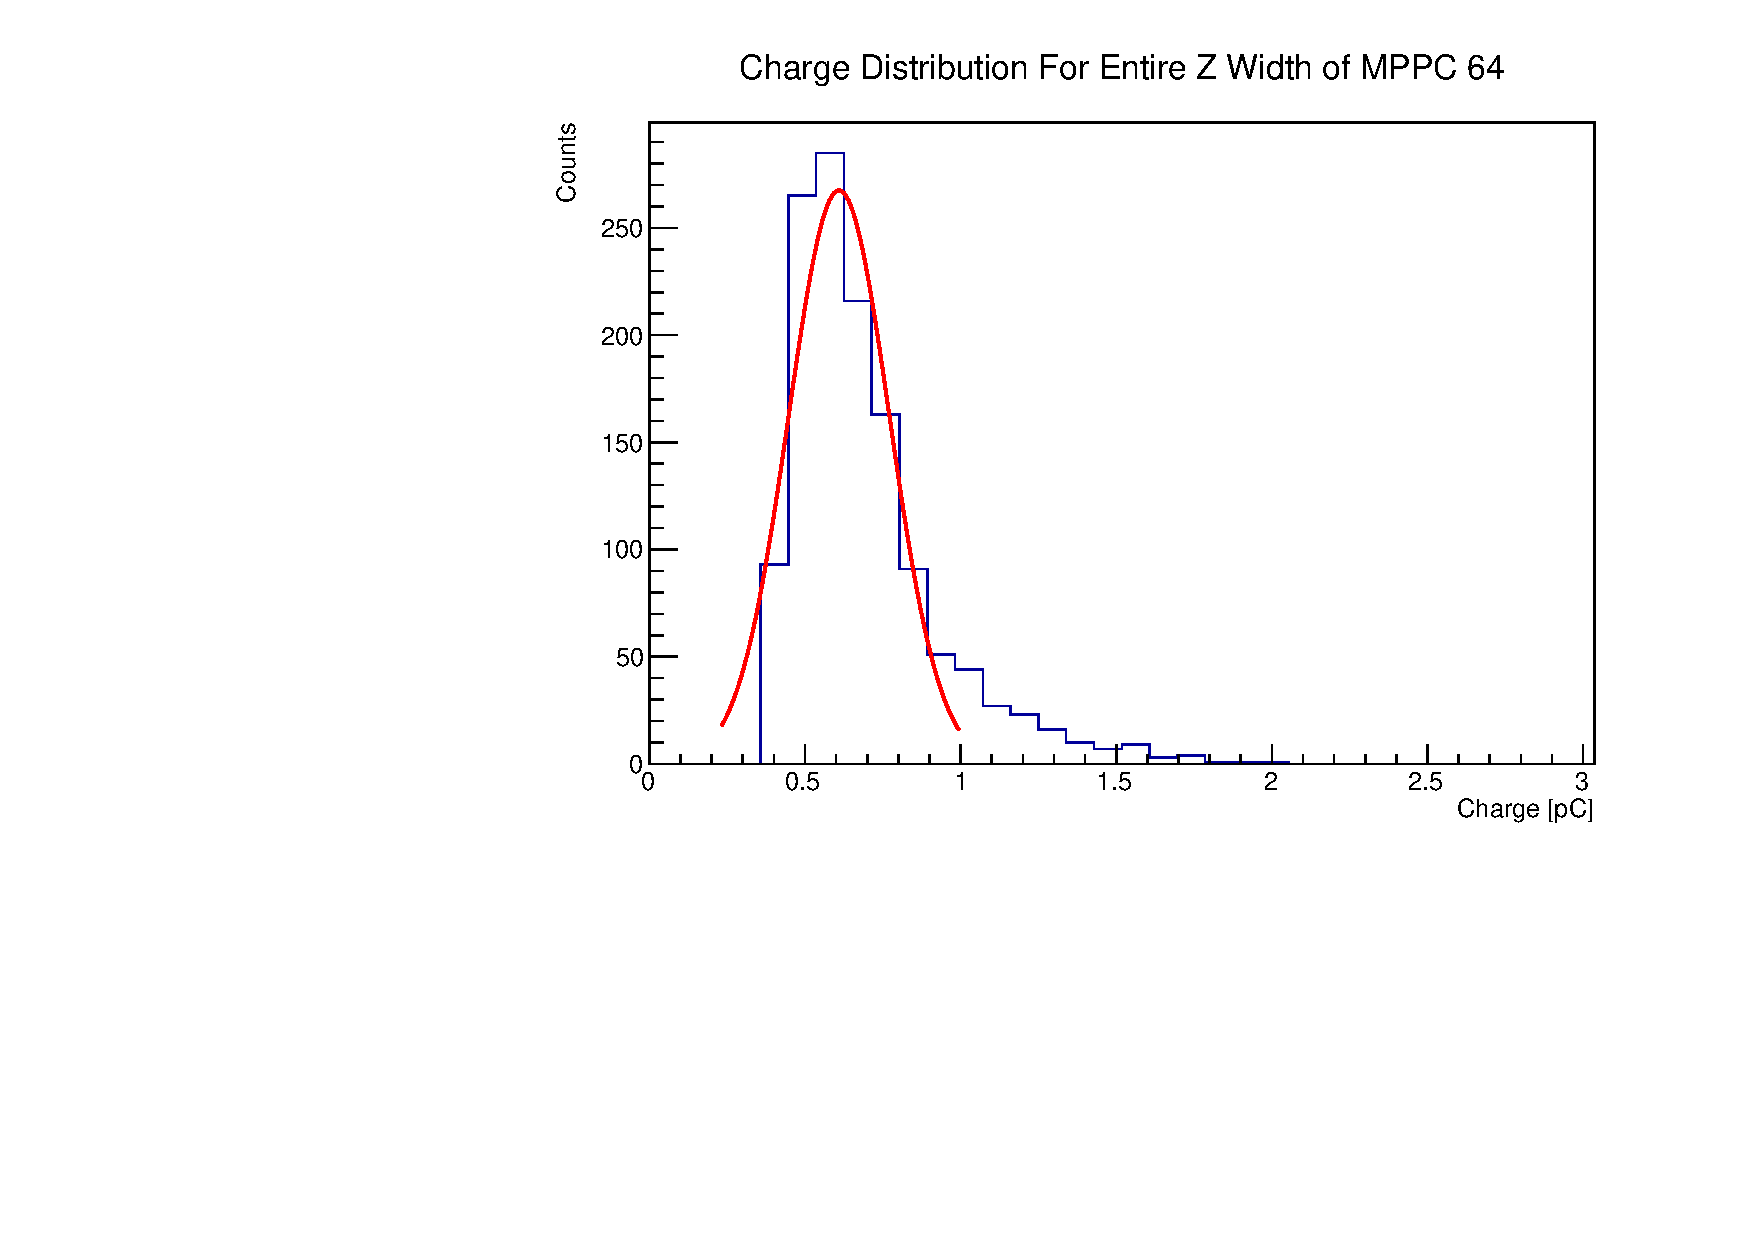
\includegraphics[width=4.35cm]{graphics/qgaindist64.pdf}
    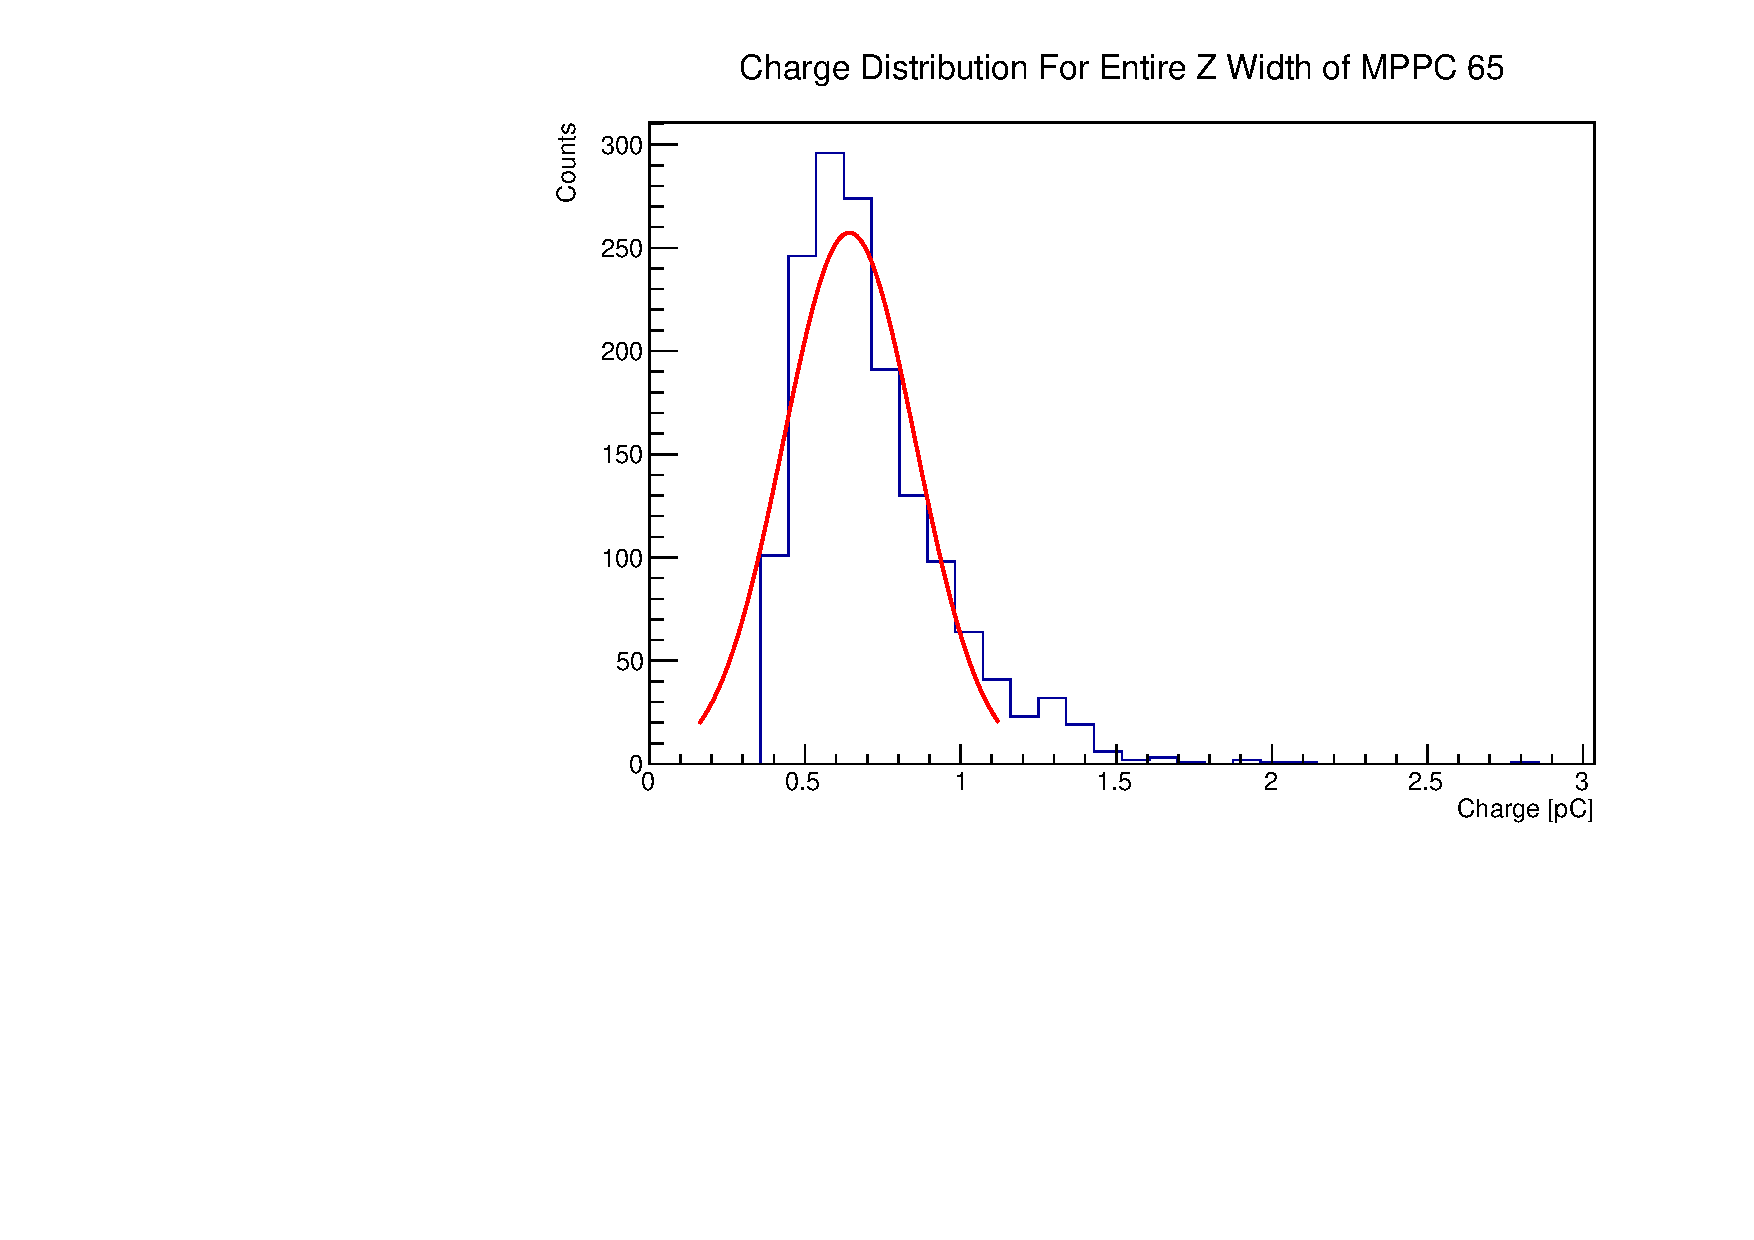
\includegraphics[width=4.35cm]{graphics/qgaindist65.pdf}
    \caption{Measured Charge Distributions And Second Iteration Gaussian Fits}
    \label{fig:qgainfits}
\end{figure}

From these plots, the average charge measurements are made through two iterations of fitting, both of which are based off of ROOT's baked-in $Fit("gaus")$ function --- this being defined as,
\begin{equation}
    Gaus[x] = A \cdot Exp\left [ - \frac{(x-\mu_{gaus})^{2}}{2\, \sigma_{gaus}^{2}} \right ]
\end{equation}
By doing two rounds of fitting, we are able use the results of our first fit -- which uses the entire data set's range -- to modify the second fit such that any systematic effects from outlying data will be removed. For this purpose, it is effective to limit the fitting range to a choice of $\mu_{gaus}\pm 2 \sigma_{gaus}$.


What then becomes immediately apparent is a strong correlation between which production lot the photodetector was manufactured in, and the resulting charge gain that is measured. Due to how this fact offers a straightforward method of generalizing predicted gain values to all detectors, we then move to sort all our single photodetector gain measurements into the appropriate one of the four data sets --- one for each production lot; labeled A,B,C, and D. 
\begin{figure}[H]
    \centering
    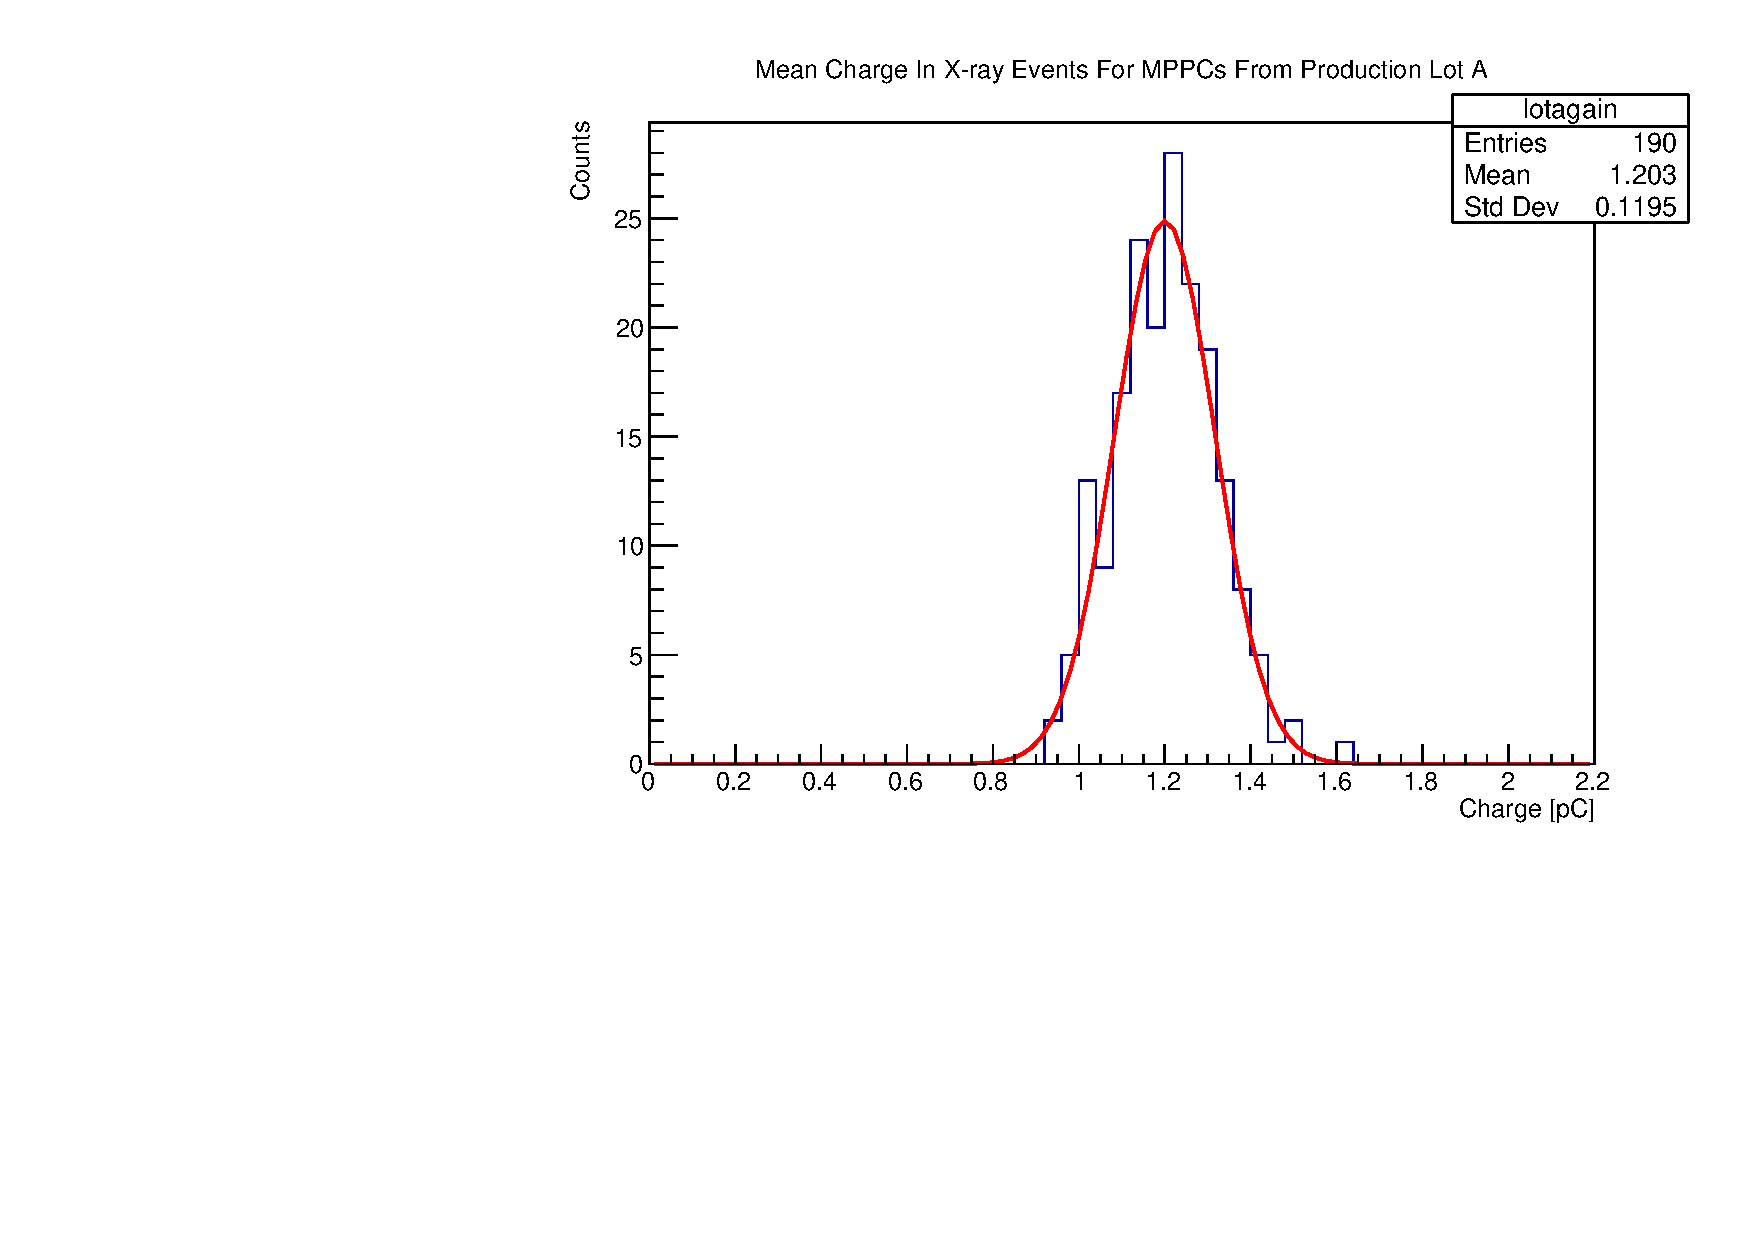
\includegraphics[width=4.25cm]{graphics/plotahistfit2.pdf}
    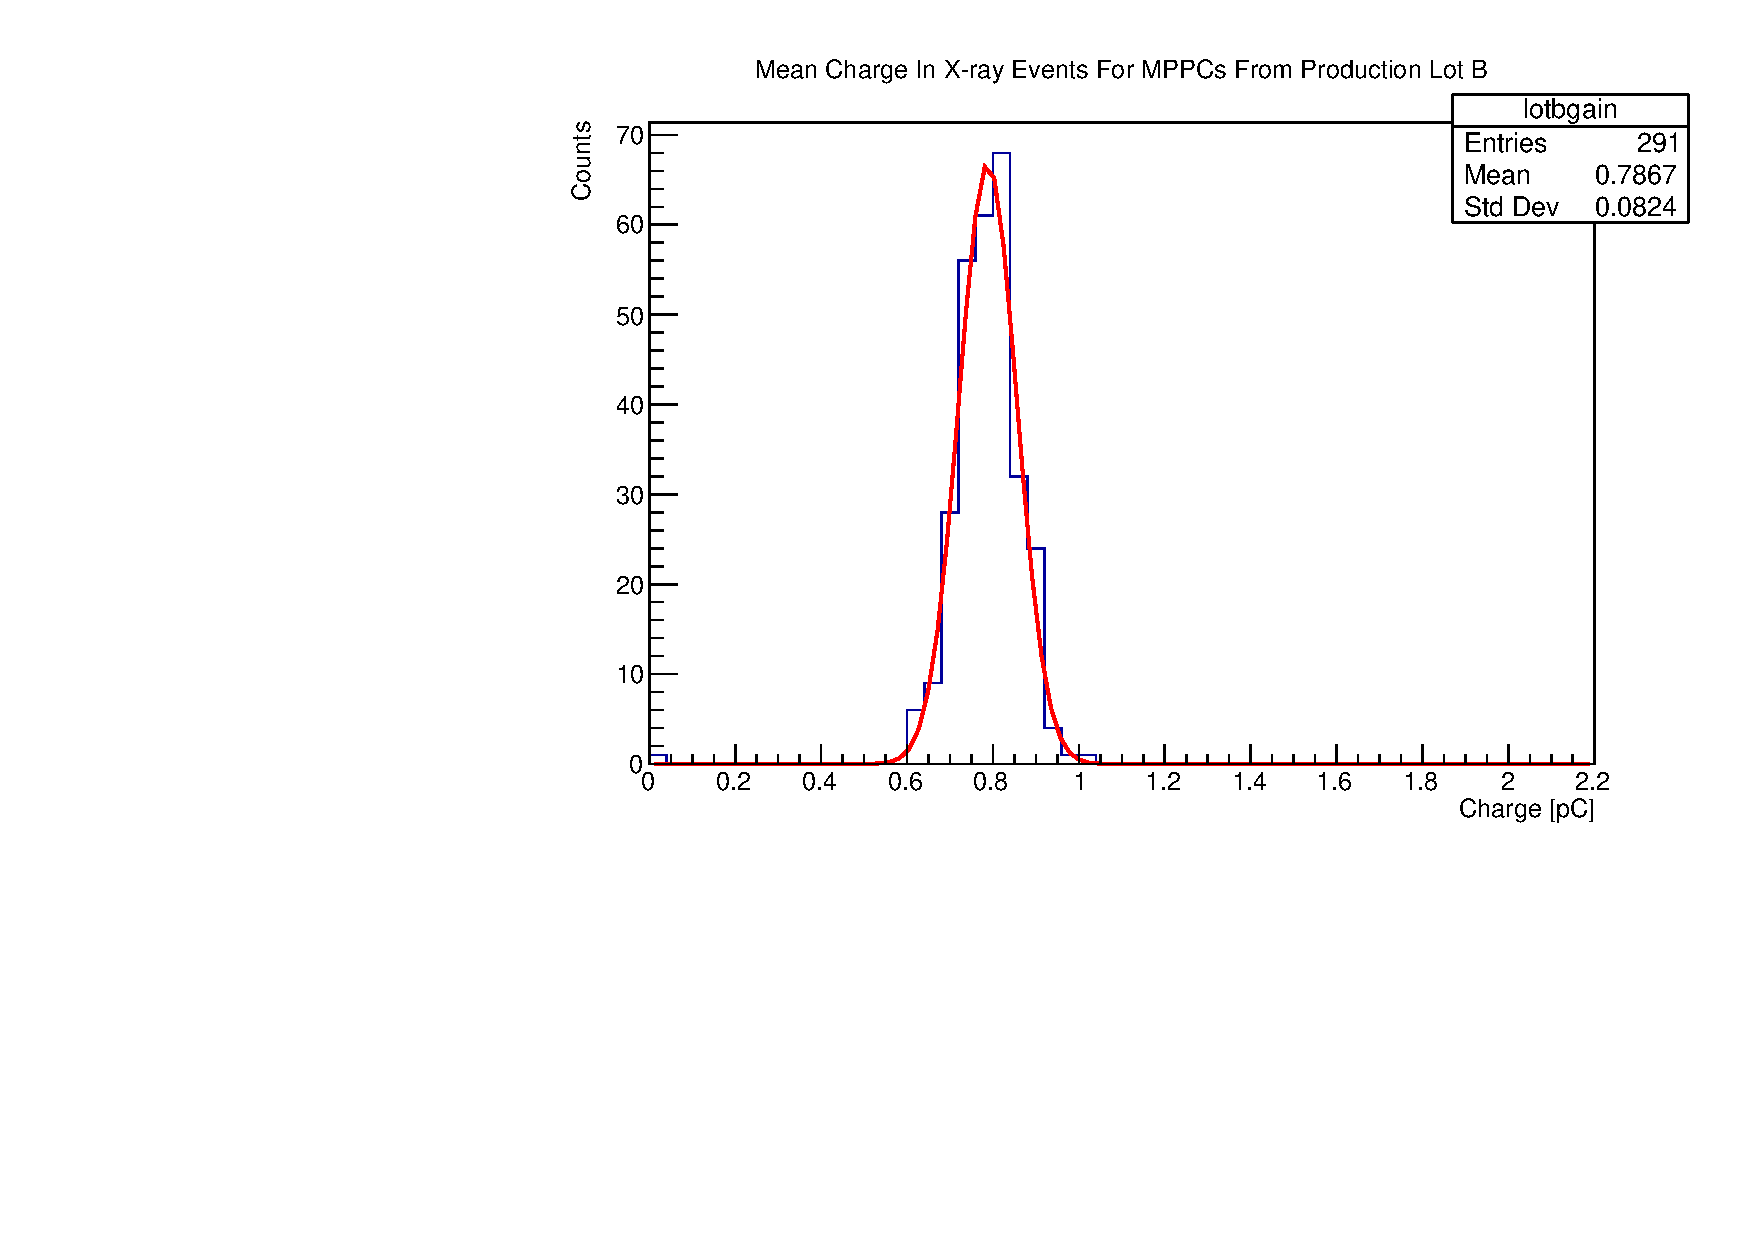
\includegraphics[width=4.25cm]{graphics/plotbhistfit2.pdf}
    
    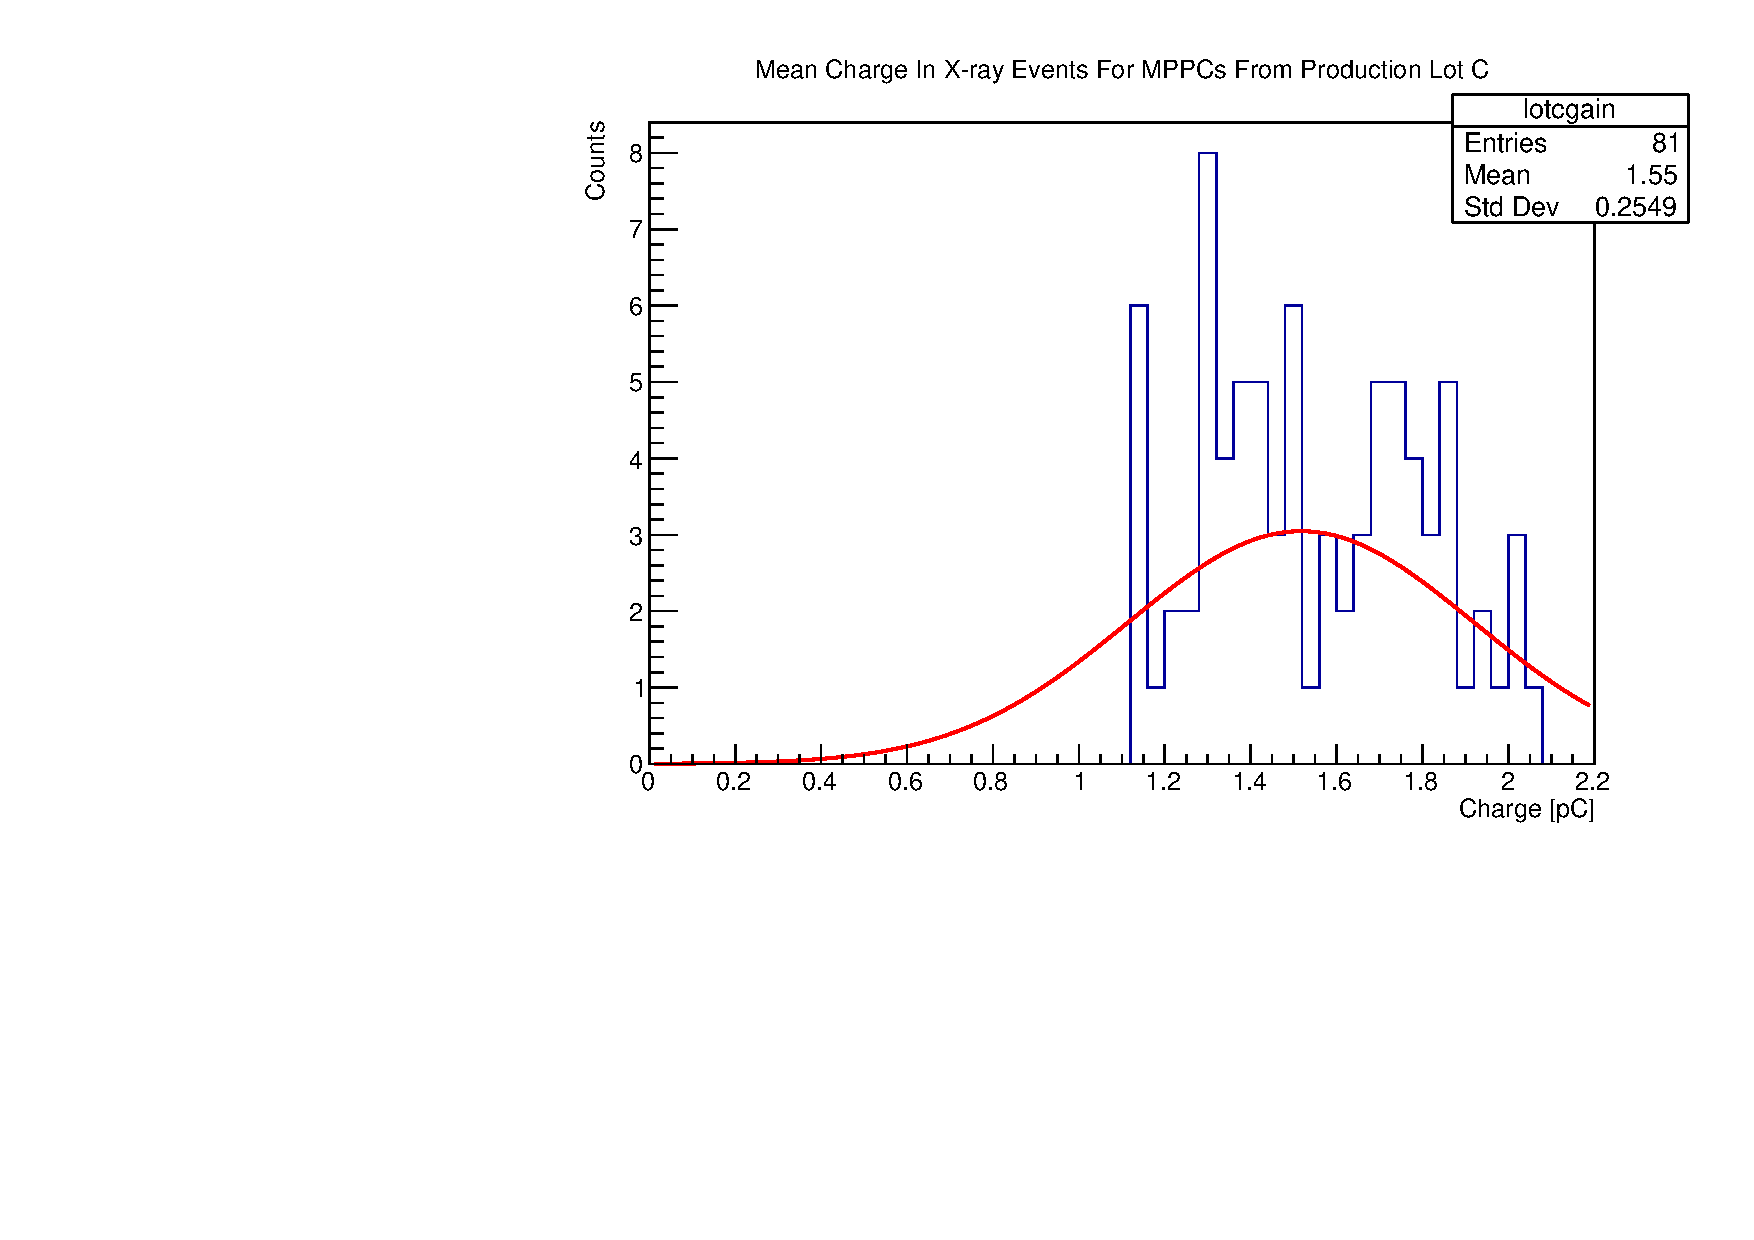
\includegraphics[width=4.25cm]{graphics/plotchistfit2.pdf}
    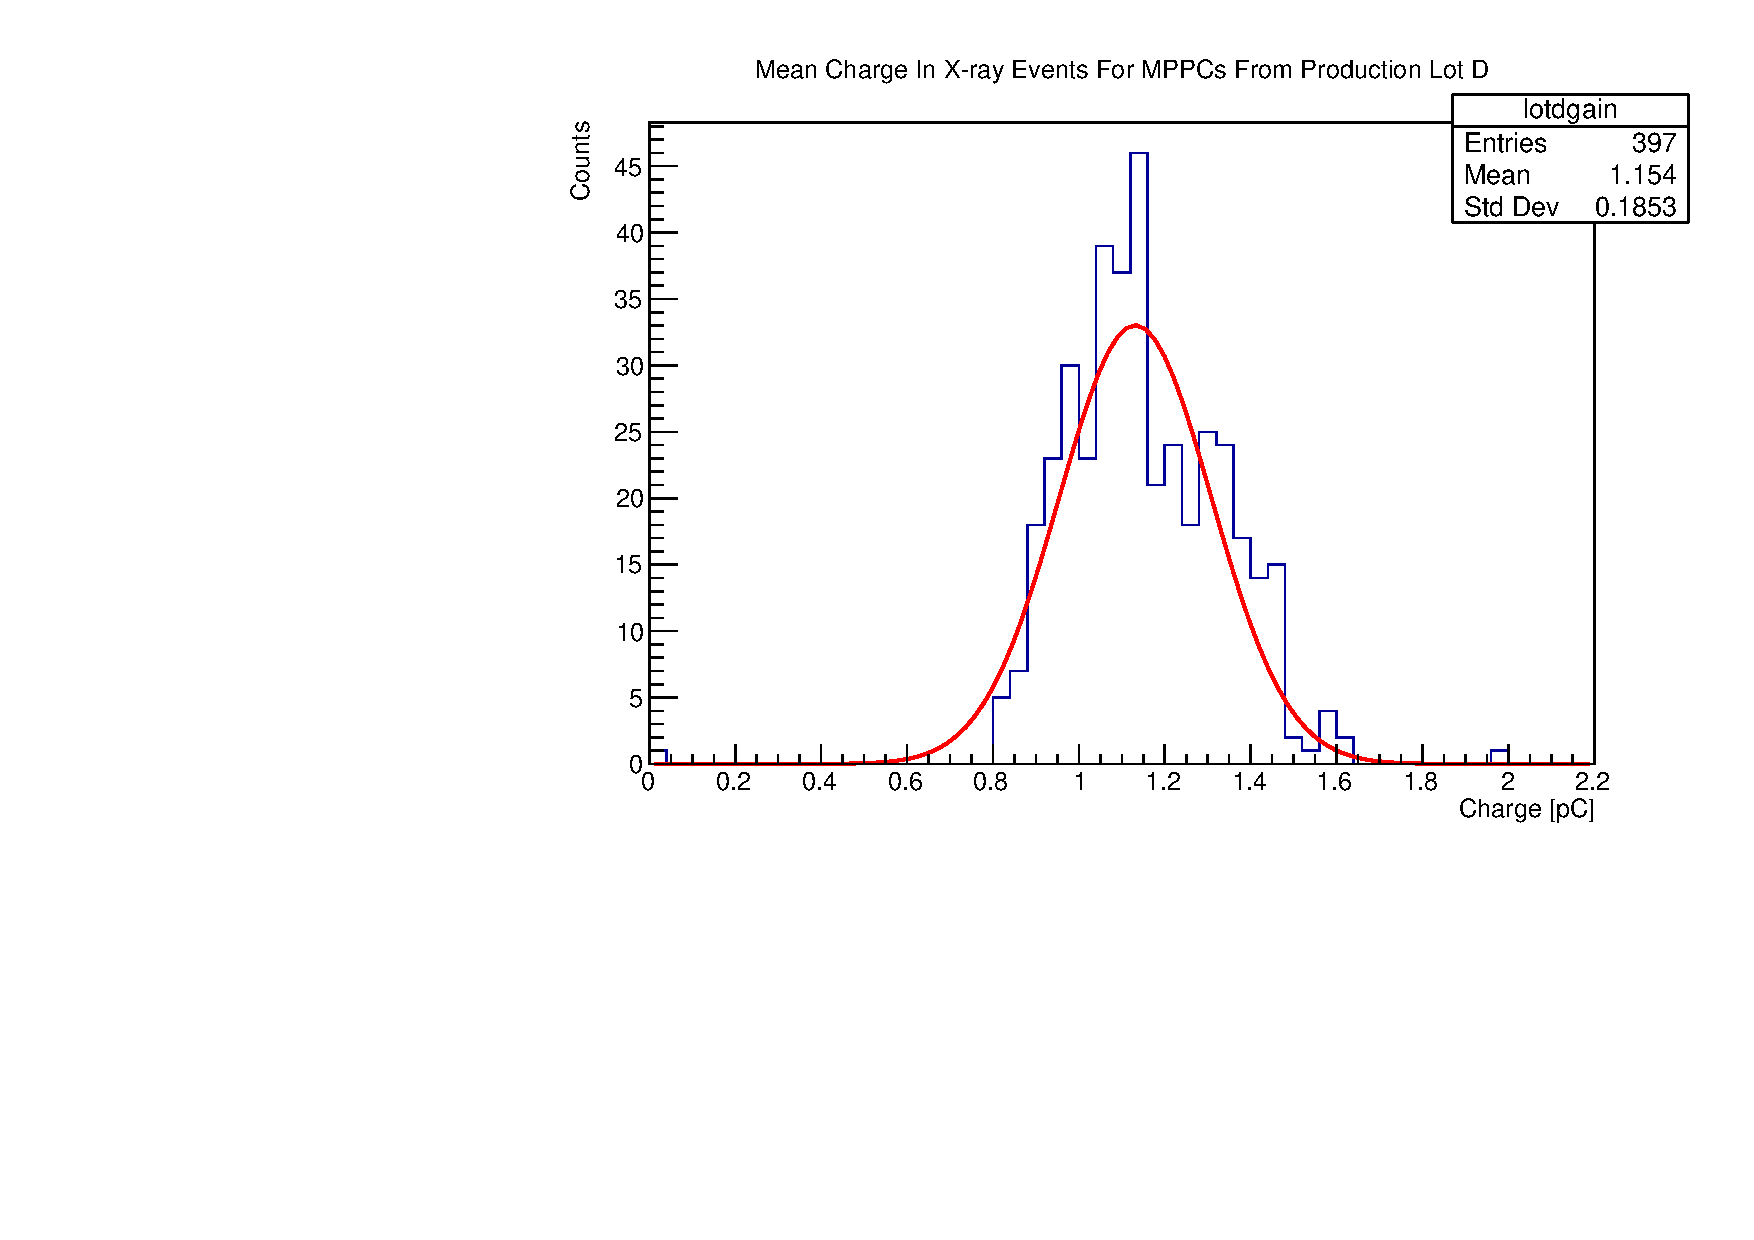
\includegraphics[width=4.25cm]{graphics/plotdhistfit2.pdf}
    \caption{Production Lot Gain Distributions With Gaussian Fits}
    \label{fig:lotgainfits}
\end{figure}

The lot-wide gain values are obtained using the same fitting approach as used in the first iteration of the single photodetector gain fitting, and the resulting values are given below in Table \ref{tab:lotgain}.
\begin{table}[H]
    \centering
    \begin{tabular}{c||c|c}
        \bf Production Lot & \bf \boldmath$\mu_{gaus}$ [pC] & \bf e\boldmath$_{\mu}$ [pC] \\
        \hline
        A & 1.200180 & $\pm$0.00931 \\
        B & 0.788079 & $\pm$0.00409 \\
        C & 1.517440 & $\pm$0.09531 \\
        D & 1.131410 & $\pm$0.01032
    \end{tabular}
    \caption{Gaussian Fitted Charge Gain For Each MPPC Production Lot}
    \label{tab:lotgain}
\end{table}

\noindent {\bf Quadrant Dependence of Charge Gain } \\
Another significant aspect in determining mean charge measurements is found to be the location within the MPPC where the X-ray event was detected. In particular, we find that there is a loss of ~10\% of the charge response in the two down-board\footnote{Down-board(DB) \& Up-board(UB) defined s.t. $|Z_{_{UB}}|>|Z_{_{DB}}|$} quadrants of a photodetector, as compared to its other two upstream quadrants.
\begin{table}[H]
    \centering
    \begin{tabular}{c||c|c}
        & $\mu$ & $\sigma_{RMS}$ \\
        \hline
        DB / UB & 0.9013 & 0.0564 \\
        Lower $\phi$ / Larger $\phi$ &  0.9951 & 0.0793
    \end{tabular}
    \caption{Ratio of Charge Measurements Between Detector Halves}
    \label{tab:halfqratiovalues}
\end{table}
The mean charge values are taken from the same data as was used in the previous calculations of whole detector gain. However, each detectors data set was split in two, depending upon the X-ray beam's position being greater than, or less than, the detector's fitted center value; the charge histograms from each of these 6mm wide collection regions are then fit to a Gaussian.
The results of dividing the mean of each detector half are plotted in Figures \ref{fig:chargeratiobtwzhalves} \& \ref{fig:chargeratiobtwphihalves}, where the chosen numerators are the down-board half for Fig. \ref{fig:chargeratiobtwzhalves} and the half at lower $\phi$ for Fig. \ref{fig:chargeratiobtwphihalves}.
\begin{figure}[H]
    \centering
    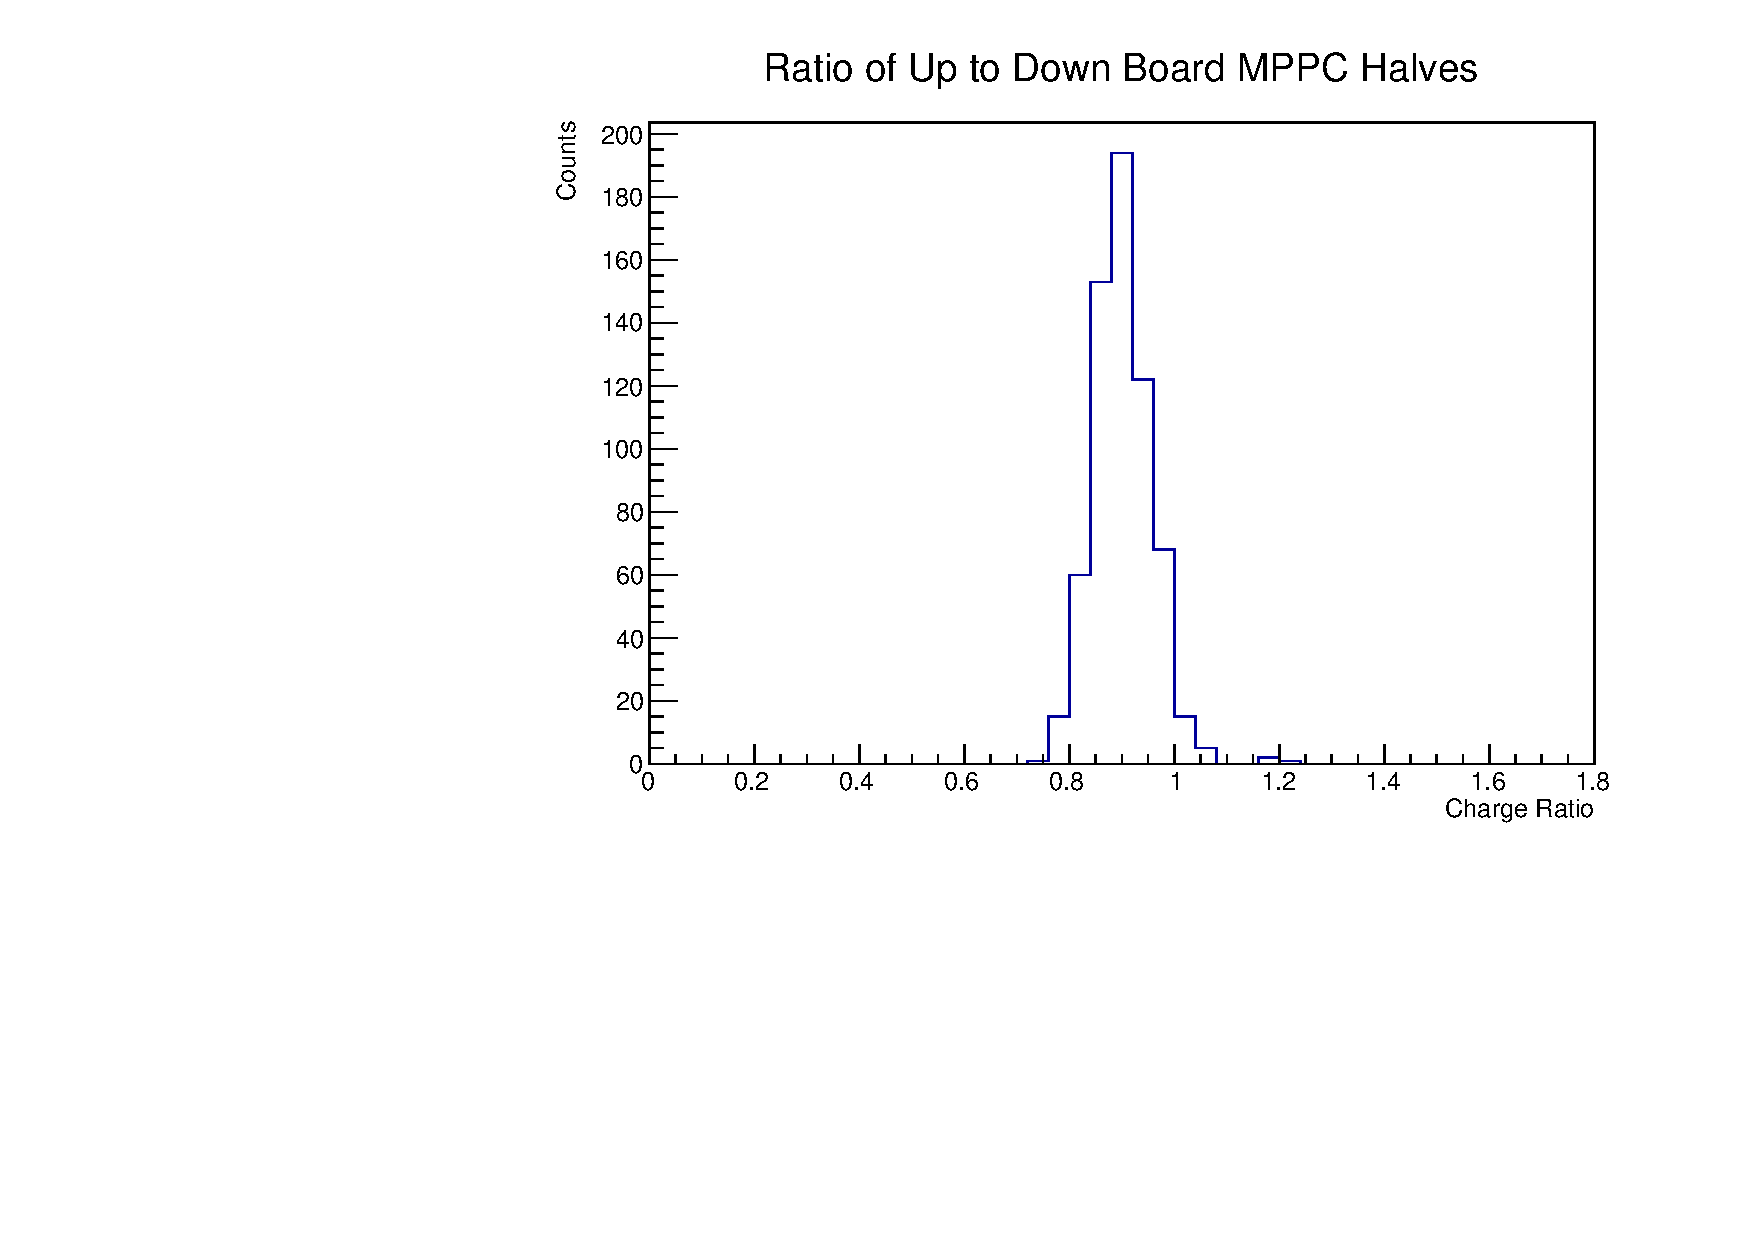
\includegraphics[width=8cm]{graphics/halfmppcqrationostats.pdf}
    \caption{Comparison of Detectors' Charge Response Relative to Z Coord. of Detection Quadrant}
    \label{fig:chargeratiobtwzhalves}
\end{figure}
\begin{figure}[H]
    \centering
    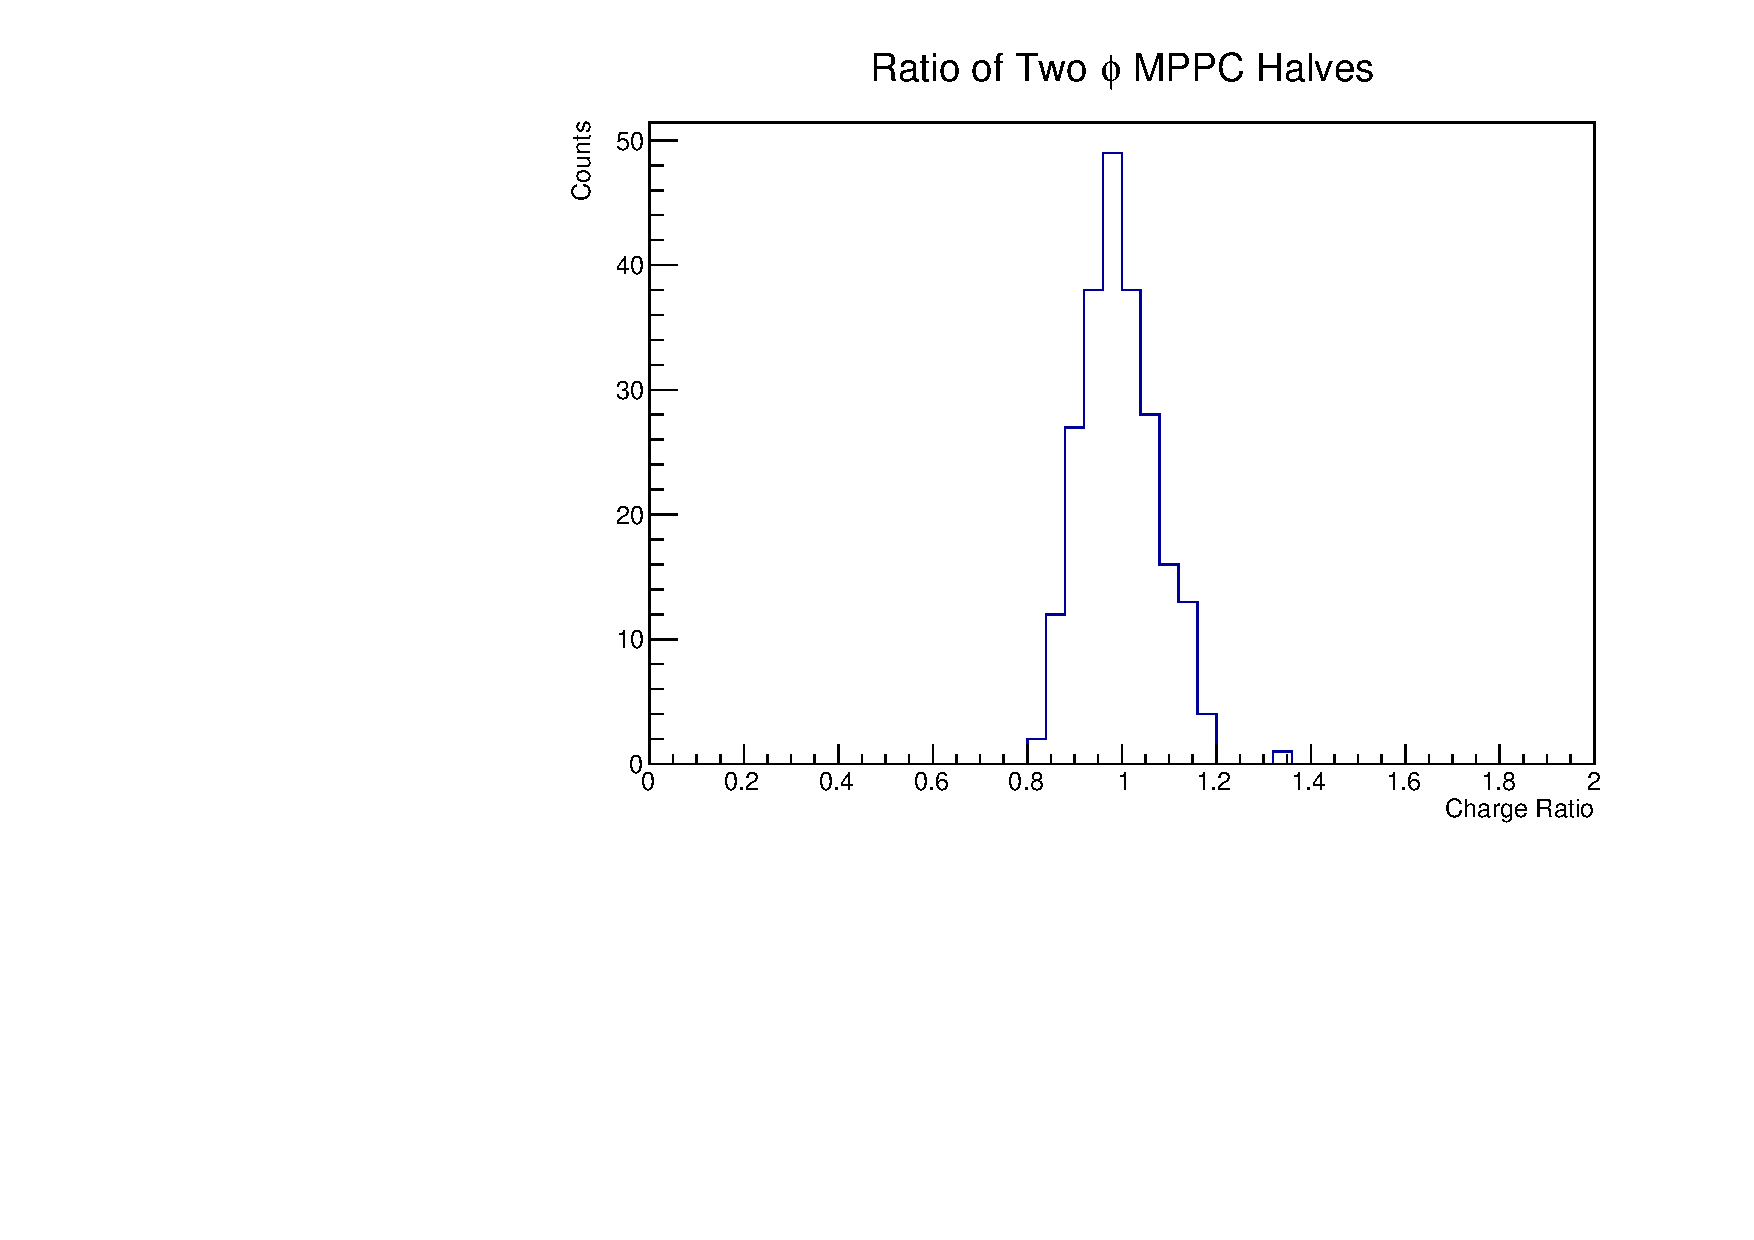
\includegraphics[width=8cm]{graphics/phihalfmppcqrationostats.pdf}
    \caption{Comparison of Detectors' Charge Response Relative to $\phi$ Coord. of Detection Quadrant}
    \label{fig:chargeratiobtwphihalves}
\end{figure}

Interestingly, we find this 10\% loss in signal is best characterised in this way -- as a percentage -- as despite the various production lots varying by up to two times the gain of one another, each lot individually still aligns to this same 10\% reduction (Table \ref{tab:lotquadqrat}.
\begin{table}[H]
    \centering
    \begin{tabular}{c||c|c}
        Lot & $\mu$ & $\sigma_{RMS}$ \\
        \hline
        A & 0.913 & 0.062 \\
        B & 0.8971 & 0.041 \\
        C & 0.9083 & 0.073 \\
        D & 0.8981 & 0.059
    \end{tabular}
    \caption{Ratio of DB / UB Charge Measurements Separated By Production Lot}
    \label{tab:lotquadqrat}
\end{table}


\subsection{Quantum Efficiency$\times$Gain} \label{QEsec}

\noindent QE$\times$gain provided by X-ray measurement \\
Gain + Cross-talk + Afterpulse $\times$QE is measured. \\
Mean charge calculation - Fitting the peak \\
Mean charge vs Z (x-ray pos) \\
Z - left and right hemisphere variation in charge response by 27\% average. \\
Mean charge variation by 30\%, and correlated with production batch number. \\



